% For pdflatex 
\documentclass [11pt]{article}

\usepackage{amssymb,amsmath,graphicx,setspace}

\usepackage[titles]{tocloft}
\setlength{\cftbeforesecskip}{-.5ex}

\usepackage{enumitem}
\setlist{topsep=.125em,itemsep=-0.05em,leftmargin=0.75cm}

\usepackage[compact]{titlesec}
\usepackage[vmargin=1in,hmargin=1in]{geometry}

\setlength{\parskip}{.1in}  
\setlength{\parindent}{0.0in}  

\usepackage[formats]{listings}
\usepackage{color}
\definecolor{mygreen}{rgb}{0.1,0.5,0.1}
\definecolor{mygray}{rgb}{0.5,0.5,0.5}
\definecolor{mymauve}{rgb}{0.58,0,0.82}
\definecolor{mygrey}{rgb}{0.3,0.3,0.1}
\lstset{
language=R,
otherkeywords={data.frame},
basicstyle=\normalsize\ttfamily, 
commentstyle=\normalsize\ttfamily,
keywordstyle=\normalsize\ttfamily,
stringstyle=\color{mymauve}, 
commentstyle=\color{mygreen},
keywordstyle=\color{blue},
showstringspaces=false, xleftmargin=2.5ex,
columns=flexible,
literate={~}{{$\sim \; \; $}}1,
alsodigit={\.,\_},
deletekeywords={on,by,data,R,Q,mean,var,family,na,options,q,weights,effects,matrix,wt,fix,distance},
}
\lstset{escapeinside={(*}{*)}} 

\usepackage[scaled=1]{zi4}

\pagestyle{headings}

\def\X{\mathbf{X}}
\def\A{\mathbf{A}}
\def\B{\mathbf{B}}
\def\C{\mathbf{C}}
\def\D{\mathbf{D}}
\def\S{\mathbf{S}}
\def\E{\mathbf{E}}
\def\I{\mathbf{I}}
\def\N{\mathbf{N}}


\def\x{\mathbf{x}}
\def\b{\mathbf{b}}
\def\u{\mathbf{u}}
\def\v{\mathbf{v}}
\def\w{\mathbf{w}}
\def\n{\mathbf{n}}
\def\p{\mathbf{p}}

\newcommand{\be}{\begin{equation}}
\newcommand{\ee}{\end{equation}} 

\newcommand{\bv}{\vspace{-0.05in} \begin{verbatim}}
\newcommand{\ev}{\end{verbatim}}

\newcommand{\blst}{\vspace{-0.035in} \begin{lstlisting}}



\newcommand{\ttt}[1]{\texttt{#1}}
\newcommand{\tab}{\hspace*{0.5in}}
\newcommand{\lift}{\vspace{-0.15in}} 


\newcommand{\tw}[1]{\texttt{#1}}
\newcommand{\bi}{\begin{itemize} \vspace*{-0.1in}}


\newcounter{exercise}
\numberwithin{exercise}{section}
\newcommand{\exnumber}{\addtocounter{exercise}{1} \theexercise \thinspace}

\def\R{R }

\sloppy

\renewcommand{\rmdefault}{ptm}

\begin{document}
\begin{center}
\Large An introduction to \R for dynamic models in biology\\
\normalsize Last compile: \today \\
\vspace{0.25in}
\large  
Stephen P. Ellner$^1$ and John Guckenheimer$^2$\\ 
${}^1$Department of Ecology and Evolutionary Biology, and \\
${}^2$Department of Mathematics \\
Cornell University, Ithaca NY 14853 \\
\normalsize 
\end{center}

\tableofcontents 

\section*{Preface}
These notes for computer labs accompany the textbook \textit{Dynamic Models in Biology} (Princeton University
Press 2006), but they can also be used as a standalone introduction to \R for
simulating dynamic models of biological systems. They are based in part on course materials 
by former TAs Colleen Webb, Jonathan Rowell and Daniel Fink (then at Cornell University), 
Lou Gross (University of Tennessee) and Paul Fackler (NC State University), and on the book 
\textit{Getting Started with Matlab} by Rudra Pratap (Oxford University Press). 
We also have drawn on the documentation built into \R.  
 
The current home for these notes is \texttt{www.cam.cornell.edu/$\sim$dmb/DMBsupplements.html},
a web page for the textbook that we maintain ourselves. If that fails, an up-to-date link should 
be in the book's listing at the publisher (\texttt{www.pupress.princeton.edu}). Parallel notes
and script files for \textsc{Matlab} are also available at those sites. 
This document was originally written at a Windows PC and may sometimes refer to Windows-specific
aspects of \R. We will be happy to make changes as these are brought to our attention.   

Sections 1-7 are an autotutorial introduction to basic \R programming (we  
generally cover them in two or three 2-hour lab sessions, depending on how much previous
experience students have had). Those sections contain many sample calculations. It is important to 
do them yourselves -- \textit{type them in at your keyboard and see what
happens on your screen} -- to get the feel of working in \R. 
Exercises in the middle of a section should be done \textit{immediately} when you 
get to them, and make sure that you have them right 
before moving on. Exercises at the ends of sections may be more 
appropriate as homework exercises. $\maltese$ marks the end of an exercise. 

Subsequent sections link to the textbook in fairly obvious ways. For example,
section \ref{MatComp} on matrix computations goes with Chapter 2 on matrix models for
structured populations, and section \ref{Mchain} goes with the Markov Chains section of Chapter 3. 
Some exercises in these sections are ``warmups'' for
exercises in the textbook, such as simple examples of agent-based 
models as a warmup for agent-based simulation of infectious disease dynamics. 

\subsection*{What is \R?}
\R is an object-oriented scripting language that combines 
\begin{itemize}
\item the \textsf{S} statistical programming language developed by John Chambers (Chambers and
Hastie 1988, Chambers 1998, Venables and Ripley 2000).
\item a user interface with a few basic menus and extensive help facilities.
\item an enormous set of functions for dynamic and statistical modeling.  
\item graphics functions for visualizing data and model output.
\end{itemize}
\R is an open-source project available at \texttt{www.cran.r-project.org}
for Windows, OS X and several flavors of Linux. Originally a research project in statistical computing (Ihaka and
Gentlemen 1996) it is now managed by an international development team and is widely used by statisticians 
and biologists. \R mostly follows version 3 of the \textsf{S} language, but some packages use version 4 features. 
\textit{These notes refer only to version 3 of} \textsf{S}. We also limit ourselves to
graphics functions in the base graphics package, rather than the more 
advanced packages \texttt{grid, lattice, ggplot2}, and do not use the Hadleyverse (google it).    

RStudio provides a GUI for \R that's similar to the one for \textsc{Matlab}. 
It's available free at \texttt{rstudio.org/download/desktop}. Many people like it. We don't.  

\textbf{Using the help system} is an essential \R skill. If you know that the \texttt{plot()}
function plots things, but you don't know exactly how to make a particular kind of plot,
type \texttt{?plot} at the R command prompt. If \texttt{plot}
doesn't do what you want, try \texttt{??plot} to get a list of other
functions that have ``plot'' as part of their name - maybe one of them will do what you need. 
Once you get the habit of using it, and get familiar with how \R help
pages are structured, the Help system is enormously helpful.  

Also, there is tons of information on the Web at message-board sites like  
\texttt{StackOverflow}. If you get an error message that you don't
understand, a useful strategy is to copy-paste that message from the console into the
search bar in your favorite web browser, and add \texttt{[R]} in front of the message 
before you do the search. Web searches can also find answers to lots of ``how do I...'' questions. 

\subsection*{Statistics in \R}
Some of the important functions and libraries (collections of functions) for data analysis
and statistical modeling are summarized in Table 
\ref{StatModelingFunctions}. The book by Venables and Ripley (2002) gives a good practical overview, and a 
list of available libraries and their contents is available at CRAN 
(\ttt{www.cran.r-project.org}, click on \ttt{Package sources}). For the most part, we are 
not concerned here with that side of \R. 

\begin{table}[t!]
\begin{tabular}{p{140pt}p{290pt}}
\hline
aov, anova & Analysis of variance or deviance\\
lm, glm &  Linear and generalized linear models\\
gam, gamm & Generalized additive models and mixed models (in \textbf{mgcv} package) \\
nls & Fit nonlinear models by least-squares (in \textbf{nls} package)\\
lmer,glmer,nlmer & Linear and nonlinear mixed-effects models (in \textbf{lme4} package) \\
nonparametric regression & Numerous functions in libraries including
\textbf{stats} (smoothing splines, loess, kernel), \textbf{mgcv, fields, KernSmooth, logspline, sm} \\
boot & Package: functions for bootstrap estimates of precision and significance \\
multiv & Package: multivariate analysis \\
survival & Package: survival analysis \\
tree & Package: tree-based regression \\
\hline 
\end{tabular}
\caption{\small{A few of the functions and add-on packages in {\bf R} for statistical
modeling and data analysis. There are \textbf{many} more, but you will have
to learn about them somewhere else.}} 
\label{StatModelingFunctions}
\end{table}

\section{Interactive calculations}
Launching \R opens the \textbf{console} window. This 
has a few basic menus at the top, whose names and content 
are OS-dependent; check them out on your own. The console window is 
also where you enter commands for \R to execute 
\textit{interactively}, meaning that the command is executed and 
the result is displayed as soon as you hit the Enter key. For example, at 
the command prompt \texttt{>}, type in \texttt{2+2} and hit Enter; you will see 
\blst
> 2+2 
[1] 4
\end{lstlisting}

To do anything complicated, the results from calculations have to be stored 
in variables. For example, type \texttt{a=2+2; a} at the prompt and you 
see
\blst
> a=2+2; a
[1] 4
\end{lstlisting}
The variable \texttt{a} has been created, and assigned the value 4. The semicolon
allows two or more commands to be typed on a single line; the second of
these (\texttt{a} by itself) tells \R to print out the value of \texttt{a}. By 
default, a variable created this way is a vector (an ordered list of numbers); 
in this case \texttt{a} is a vector length 1, which acts just like a number. 

Variable names in \R must begin with a letter, and followed by alphanumeric 
characters (i.e., numbers and letters). Long names can be broken up using a period, as in
\texttt{very.long.variable.number.3}, or by the underscore character  
as in \texttt{make\_iteration\_matrix}. However, you cannot use blank space as a separator
in variable names; \texttt{new population size=3} will get you an error message.  It is
currently fashionable to use ``camel case'', as in \texttt{newPopulationSize=3} -- variable names
start with a lower-case letter, and upper case is used to mark a separation. \R is case 
sensitive: \texttt{Abc} and \texttt{abc} are \textbf{not} the same variable. 

\textbf{Exercise\exnumber} Here are some variable names that cannot
be used in \R; explain why: \texttt{cell maximum size; 4min; site\#7 .} $\maltese$ 

Calculations are done with variables as if they were numbers. \R uses  
\verb! +, -, *, /, and ^ !
for addition, subtraction, multiplication, division and 
exponentiation, respectively. For example enter
\blst
> x=5; y=2; z1=x*y; z2=x/y; z3=x^y; z2; z3
\end{lstlisting}
and you should see
\blst
[1] 2.5
[1] 25
\end{lstlisting}

Even though the variable values for \texttt{x, y} were not displayed, \R ``remembers" that values have 
been assigned to them. Type \verb! > x; y ! to display the values. 

If you mis-enter a command, it can be edited instead of starting again from 
scratch. The \thinspace $\uparrow$ \thinspace key recalls previous 
commands to the prompt. For example, you can bring back the next-to-last command and edit it to
\blst
> x=5 y=2 z1=x*y z2=x/y z3=x^y z2 z3 
\end{lstlisting}
so that commands are not separated by a semicolon. Then press Enter, 
and you will get an error message. 

You can do several operations in one calculation, such as 
\blst
> A=3; C=(A+2*sqrt(A))/(A+5*sqrt(A)); C
[1] 0.5543706
\end{lstlisting}

The parentheses are specifying the order of operations. The command
\\
\hspace*{1in} \texttt{> C=A+2*sqrt(A)/A+5*sqrt(A)} \\
gets a different result -- the same as \\
\hspace*{1in} \texttt{> C=A + 2*(sqrt(A)/A) + 5*sqrt(A)}.
\\

The default order of operations is: (1) Exponentiation, (2) multiplication 
and division, (3) addition and subtraction. 
\blst
> b = 12-4/2^3          gives    12 - 4/8 = 12 - 0.5 = 11.5
> b = (12-4)/2^3        gives    8/8 = 1
> b = -1^2              gives    -(1^2) = -1
> b = (-1)^2            gives    1 
\end{lstlisting}
In complicated expressions it's best to \textbf{use parentheses to specify 
explicitly what you want}, such as \verb! > b = 12 - (4/(2^3)) ! 
or at least \verb! > b = 12 - 4/(2^3) !. 

\begin{table}[tb]
\caption{Some of the built-in mathematical functions in {\bf R}. You can
get a more complete list from the Help system: ?Arithmetic for simple, 
?log for logarithmic, ?sin for trigonometric, and ?Special for special functions.} 
\vspace{0.1in}
\begin{tabular}{p{140pt}p{290pt}}
\hline
abs(x) & absolute value \\
cos(x), sin(x), tan(x) &  cosine, sine, tangent of angle x in radians\\
exp(x)  & exponential function  \\
log(x)  & natural (base-e) logarithm \\
log10(x) &  common (base-10) logarithm \\
sqrt(x)  &  square root \\
\hline 
\end{tabular}
\label{MathFunctions}
\end{table}

\R also has many \textbf{built-in mathematical functions} that operate on variables
(see Table \ref{MathFunctions}). 

\textbf{Exercise\exnumber}: Have \R compute the values of 
\begin{enumerate}
\item[(a)] $\dfrac{2^7}{2^7 - 1}$and compare it with $\left( {1 - \dfrac{1}{2^7}} 
\right)^{ - 1}$  
\item[(b)] $\sin(0.25) + \cos(2\pi/7)$ (\texttt{pi} is pre-defined in R to equal the mathematical constant $\pi$).   
\item[(c)] $\dfrac{2^7}{2^7 - 1}+\sin(0.25)$, using cut-and-paste to 
assemble parts of your past commands. $\maltese$ 
\end{enumerate}

\textbf{Exercise\exnumber}: Do an Apropos on \texttt{sin} via the Help
menu, to see what it does. Next do \\
\hspace*{1in} \ttt{??sin} \\
and see what that does (answer: ??sin pulls up all help pages that
include 'sin' anywhere in their title or text. Apropos just searches 
function names for 'sin'.) Note: on a Mac you need to do Apropos at
the command line, as in \texttt{apropos('sin')}. $\maltese$ 

\textbf{Exercise\exnumber} Use the Help system to find out what
the \texttt{hist} function does, by typing \texttt{?hist} at the command prompt. 
Prove that you have succeeded by doing the following: use the command \ttt{y=rnorm(5000)} to generate
a vector of 5000 random numbers with a Normal distribution, and then
use \ttt{hist} to plot a histogram of the values in \ttt{y} with about 20 bins. Why did we say ``about 20''
rather than ``exactly 20''? Find the answer in the Help page for \texttt{hist}. $\maltese$ 


\section{First interactive session: linear regression \& a population growth model}
To get a feel for working in \R we'll use linear regression to fit a population growth model
to data. Below are some data on the growth of a laboratory population 
of the green alga \textit{Chlorella vulgaris}. This experiment was run during the system-design 
phase of the study reported by Fussmann et al. (2000). 

time(days) =     0   1   2   3   4   5    6   7    8    9    10   12   14   21   25   32   33\\
$10^5$ cells/ml: 1.1 1.4 4.1 5.5 5.4 10.7 6.0 22.0 19.8 26.7 31.4 30.9 27.1 40.2 36.1 36.8 31.6 \\
 
To analyze these data in \R, first enter them\footnote{To save yourself some time, you can cut-and paste
the lines below from the PDF file into the R console.}
as numerical \textit{vectors}: 
\blst
tvals=c(0,1,2,3,4,5,6,7,8,9,10,12,14,21,25,32,33); 
cvals=c(1.1,1.4,4.1,5.5,5.4,10.7,6.0,22.0,19.8,26.7,31.4,30.9,27.1,40.2,36.1,36.8,31.6);
\end{lstlisting}
The function \texttt{c()} \textit{combines} 
the individual numbers into a vector; enter \ttt{tvals} in the console to see this.  

To see a histogram of the population counts enter \verb! > hist(cvals) !
which opens a graphics window and displays the histogram. There are \textbf{many} other 
built-in statistics functions, for example \texttt{mean(cvals)} gets you 
the mean, \texttt{sd(cvals)} and \texttt{median(cvals)} return the standard deviation and median,
respectively. 

To see how the algal population increased over time,  
\blst
> plot(tvals,cvals) 
\end{lstlisting}
creates a plot. By default, only the points are plotted. To connect the points, you can
ask for a plot of type ``l'' for ``line'', 
\blst
> plot(tvals,cvals,type="l")
\end{lstlisting}
or of types ``b'' or ``o'' (for ``both'' and ``overlay'') to plot the points and connecting
lines. \textbf{Try all of these right now.} 

The population seems to exhibit sigmoid growth, up to some maximum density. A simple
model often fitted to such growth curves is 
\be
x(t+1)=R x(t) (1-b x(t))
\label{dl}
\ee
which is sometimes called the ``discrete logistic'' model. To generate solutions of
this model we need three things: values for $R$ and $b$, and a starting density $x(0)$. 
How can we get these? Well, when $x$ is small, equation \eqref{dl} says $x(t+1) \approx R x(t)$, 
and the solution to $x(t+1)=R x(t)$ is exponential growth:
\be
x(t)=x(0)R^t \quad \Rightarrow \quad \log x(t) = \log x(0) + t \log R.    
\ee
So if we fit a straight line to the initial part of the data, the slope will 
be an estimate of $\log R$, and the intercept will be an estimate
of $\log x(0)$. So let's plot the log-transformed data: 
\blst
> plot(tvals,log(cvals),xlab="Time (days)",ylab="log Chlorella density");  
\end{lstlisting}
Leave this plot on the screen -- we'll be adding to it later. 

My eye suggested using the first 5 data points to fit our straight line for the initial
exponential growth phase. To fit the line by linear regression, we use the
\texttt{lm()} function to create a linear model:
\blst
> y=log(cvals[1:5]); x=tvals[1:5]; 
> fit = lm(y~x)
\end{lstlisting} 
The effect of \ttt{[1:5]} in the first line is to ``pull out'' only the first 5 entries of
cvals and tvals; we'll learn more about this later. The second line 
produces no output but it has created \texttt{fit}  
as an \textbf{object}, i.e. a multi-part data structure holding the results of the 
linear regression analysis. Unlike a typical statistics package, 
\R rarely produces summary output automatically. Data analysis in \R is done by creating a 
model, and then giving additional commands to extract information 
or display results graphically.

The command \ttt{summary(fit)} prints a summary of the results in the console window. 
A model object like \ttt{fit} is set up so that the \texttt{summary} function 
can ``see'' that \texttt{fit} was created by \texttt{lm} and produces an appropriate
summary for an \texttt{lm} object: 

\blst
Call: lm(formula = y ~ x)

Residuals:
       1        2        3        4        5 
-0.04138 -0.25527  0.36420  0.20292 -0.27048 

Coefficients:
            Estimate Std. Error t value Pr(>|t|)  
(Intercept)   0.1367     0.2505   0.546   0.6233  
x             0.4550     0.1023   4.449   0.0211 *
---
Signif. codes:  0 '***' 0.001 '**' 0.01 '*' 0.05 '.' 0.1 ' ' 1 

Residual standard error: 0.3234 on 3 degrees of freedom
Multiple R-Squared: 0.8684,     Adjusted R-squared: 0.8245 
F-statistic: 19.79 on 1 and 3 DF,  p-value: 0.02113 
\end{lstlisting}
If you've had a statistics class, all of the above should make sense
to you. But for right now, the only things we need are the estimated
intercept (0.1367) and slope (0.4550). 

\begin{figure}[t]
\centerline{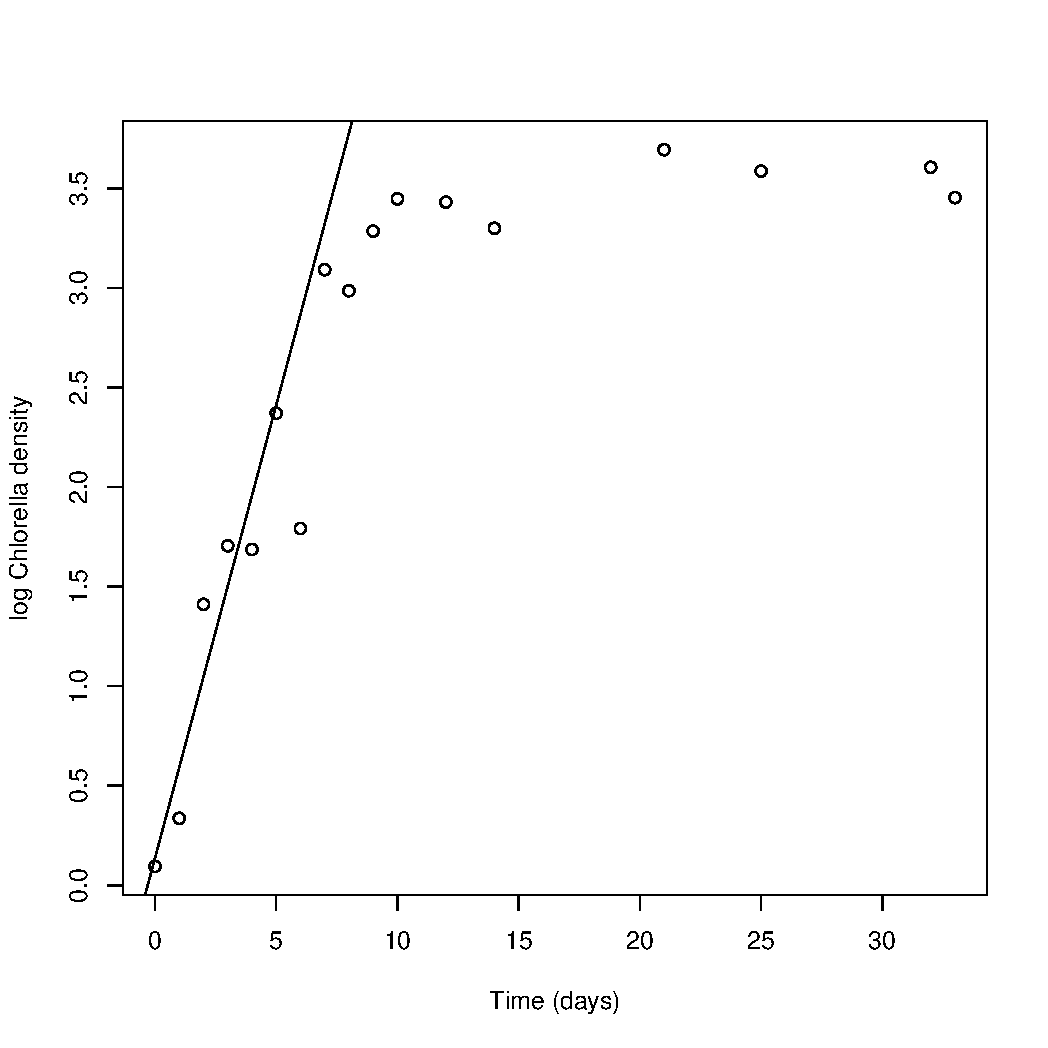
\includegraphics[width=4in]{figures/Session1Fig1.pdf}}
\caption{\small{Graphical summary of regression analysis for log \textit{Chlorella} density as
a function of time in days.}}
\label{Session1.Fig1}
\end{figure}

The regression line can be added to the data plot by 
another function that takes \texttt{fit} as its input: 
\blst
> abline(fit)
\end{lstlisting}
This gives the plot shown in Figure \ref{Session1.Fig1}. 

You can also ``interrogate'' fit directly. Type 
\verb! > names(fit) ! to get a list of the components of \texttt{fit}. 
\blst
 [1] "coefficients"  "residuals"     "effects"       "rank"         
 [5] "fitted.values" "assign"        "qr"            "df.residual"  
 [9] "xlevels"       "call"          "terms"         "model" 
\end{lstlisting}
Components of an object are extracted using the ``\$'' symbol. For
example \texttt{>fit\$coefficients} yields the regression 
coefficients 
\blst
(Intercept)           x 
  0.1366926   0.4550453 
\end{lstlisting}
We can use those to get two of the estimates that we need:
\blst
x0=exp(fit$coef[1]); R=exp(fit$coef[2]); 
\end{lstlisting}
Note that ``coefficients'' was abbreviated but \R figured out what you meant,
because no other component of \ttt{fit} started with \ttt{coef}.  

We still need to estimate $b$. Looking at the data, the value of $x(t)$ in the model 
should stop growing when $x(t)$ is about 35. That is, $x(t)=35$ then we should get $x(t+1)=35$ also. 
Substituting $x(t)=35$ and $x(t+1)=35$ into equation \eqref{dl}, we get $35=35R(1-35b).$ A bit
of algebra turns this into $35b=1-\dfrac{1}{R}$, so we have
\blst
> b=(1-1/R)/35; b 
\end{lstlisting} 

\textbf{Exercise \exnumber} 1-1=0, and (0/R)/35=0. So why does \ttt{b=(1-1/R)/35}
not give $b=0$? $\maltese$ 

\textbf{Exercise\exnumber} When we did \texttt{plot(tvals,log(cvals))} the $x$ and $y$ axis labels
were specified using the \texttt{xlab} and \texttt{ylab} arguments. 
Do \texttt{?plot} to figure out how to add a title to the plot using the \texttt{main} argument, 
so that the plot title is \textbf{Algal population growth}.   $\maltese$ 

\textbf{Exercise\exnumber} Now, figure out how to use the \texttt{pch} and \texttt{col} arguments
so that the data are plotted as green squares. You can use \texttt{?plot} and \texttt{?par} to 
find out about \texttt{pch} and \texttt{col}.  $\maltese$ 

\section{Scripts and data files}
Modeling and complicated data analyses are more easily done  
using \textit{scripts}: a series of commands stored in a text file. 
The Windows and OS X versions of \R include a basic  
script editor (accessed via the \textbf{file} menu on the console),
but you can also use an external text editor.  

Most scripts for working with models or data follow a simple pattern:
\begin{enumerate}
\item ``Setup'' statements.
\item Input some data from a file or the keyboard.
\item Carry out the calculations that you want.
\item Print the results, graph them, or save them to a file. 
\end{enumerate}

For example, a script file might
\begin{enumerate}
\item Load some packages, or run another script file that 
creates some functions (more on functions later). 
\item Read in from a text file the parameter values for a predator-prey model, and
the numbers of predators and prey at time $t=0$.
\item Calculate the population sizes at times $t=1,2,3,\ldots,T$.
\item Graph the results and save the graph as a PDF file for including
in your term project. 
\end{enumerate}
As a first example, the file \textbf{Session1.1.R} has the commands from the interactive 
regression analysis. \textbf{Important:} before working with an example file, create 
a personal copy in some location on your own computer. We will refer to this location
as your \textit{temp folder}. At the end of a lab session 
you \textbf{must} save files onto some transportable medium (e.g. a flash drive) 
or email them to yourself.  

Open \textit{your copy of} of \textbf{Session1.1.R}, using \textbf{File/Open Script}
from the console menu. On the \textbf{Edit} menu of the script editor,
select \textbf{Run All}. This equivalent to copying the
whole script and pasting it into the console window, so the commands are all 
executed and a graph is displayed with the results. The \texttt{source} function  
runs an entire script file without copying it to the console, e.g. 
\blst
> source("c:/temp/Session1.1.R")
\end{lstlisting}
Source'ing can also be done in point-and-click fashion 
via \textbf{File/Source R code} on the console window. 

Another important time saver is loading data from a text file. Get   
copies of \textbf{Session1.2.R} and \textbf{ChlorellaStart.txt} 
to see an example of how this can be done. In \textbf{ChlorellaStart.txt},
time and algal density are entered as two columns of a data matrix. Then 
instead of typing these in by hand, the command
\blst
X=read.table("c:/temp/ChlorellaStart.txt")
\end{lstlisting}
reads the data file and puts the data values into the variable 
\texttt{X}. Note that the path to the data file has to 
be specified; you need to edit the script so that it uses the correct path to your data file.  
In the console window, do  
\blst
> X
\end{lstlisting}
to see that X has been loaded into \R as a data matrix with two columns. \ttt{V1} and
\ttt{V2} are ``default'' variable names that \R has assigned to the two columns. 

The variables are then extracted from \ttt{X} with the commands
\blst
tvals=X[,1]; cvals=X[,2];
\end{lstlisting}
These are shorthand for ``tvals = everything in column 1 of X'', and 
``cvals = everything in column 2 of X'' (you'll learn about working with  
matrices later). The rest is the same as before, with some additions
that specify axis labels and a title.

\textbf{Exercise\exnumber} Make a copy of \textbf{Session1.2.R} under a new 
name, and modify the copy so that it plots algal density (without log tranformation) 
versus time, does linear regression of algal density on time, and plots the 
data appropriately. As in \textbf{Session1.2.R}, use only
the first 5 data points for the linear regression. You should end up with a graph sort 
of like Figure \ref{Session1Fig2}. $\maltese$ 

\begin{figure}[t]
\centerline{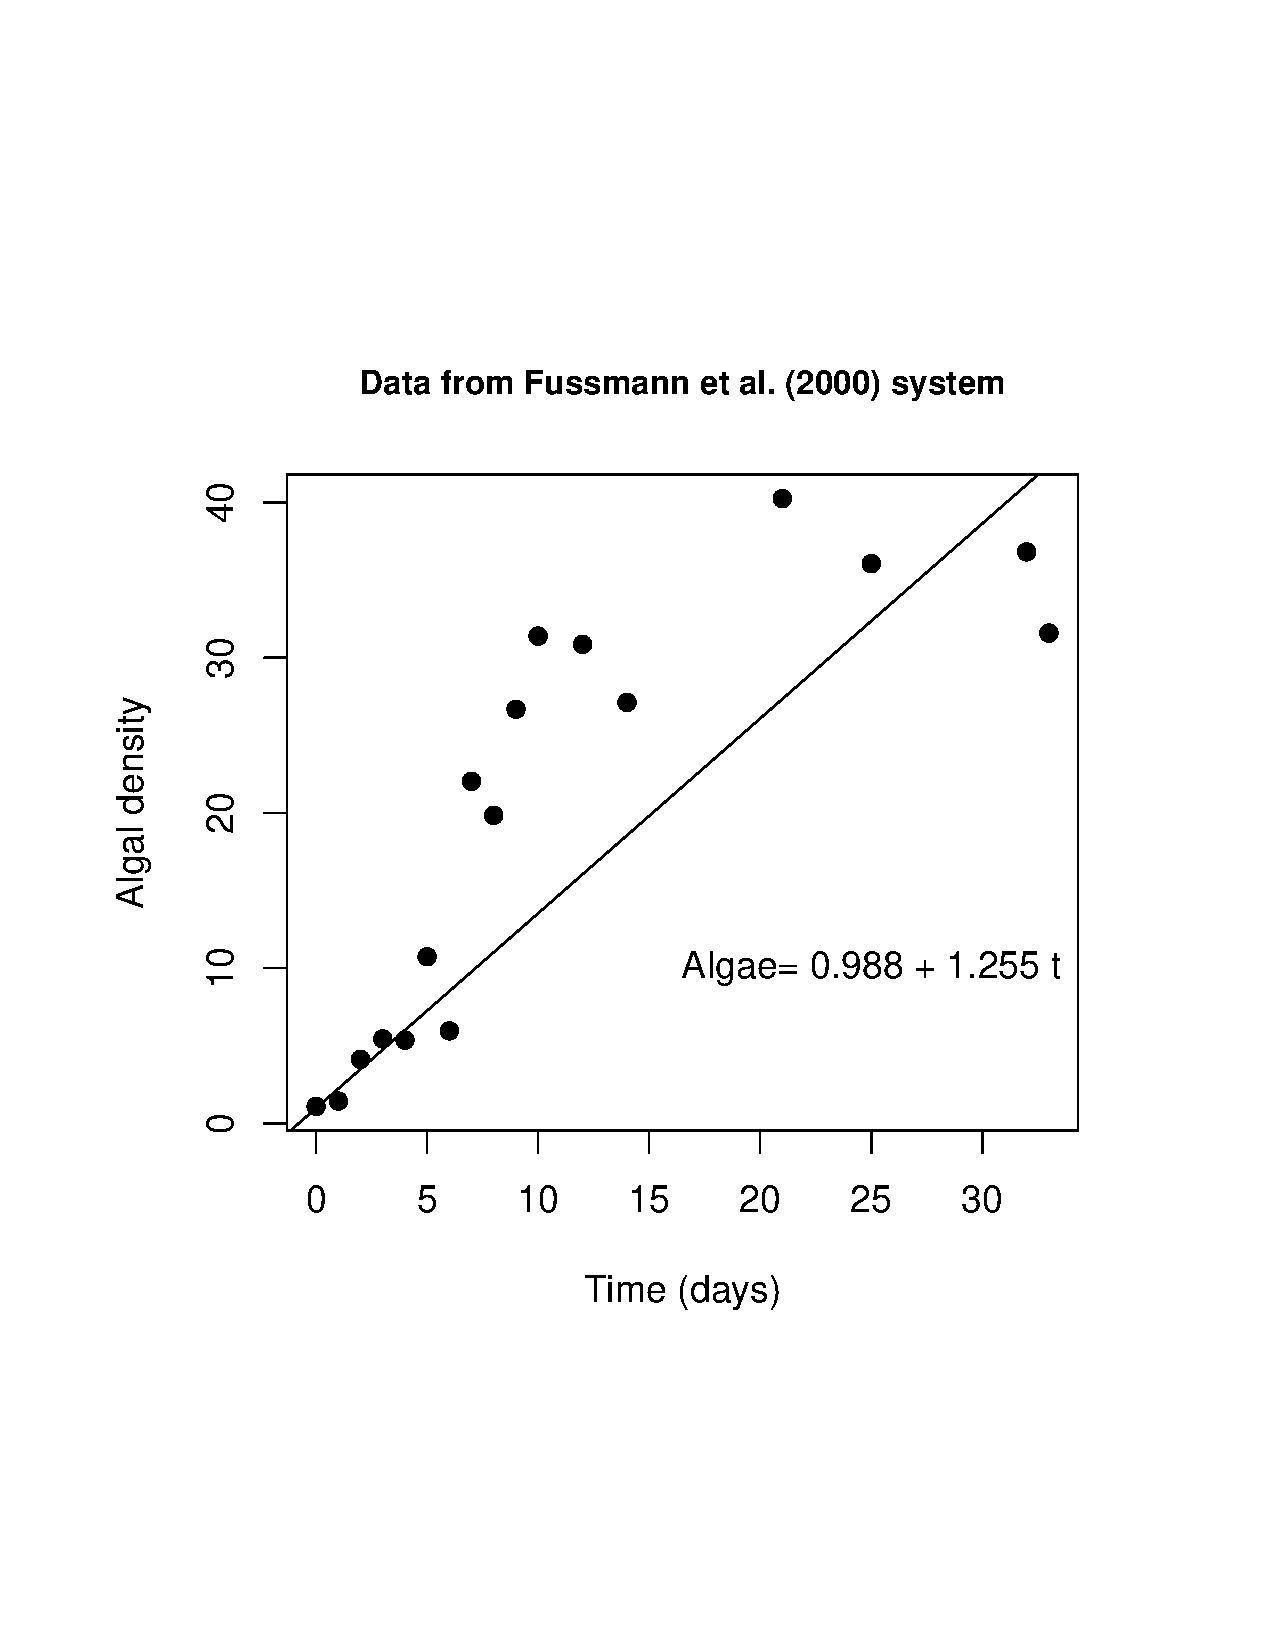
\includegraphics[width=3.5in]{figures/Session1-Fig2.pdf}}
\caption{\small{Graphical summary of regression analysis without log transformation.}}
\label{Session1Fig2}
\end{figure}

\textbf{Exercise\exnumber} Run \textbf{Session1.2.R}, then enter the command 
\ttt{plot(fit)} in the console. \R will tell you that it is ``Waiting to
confirm page change'' -- help it out by clicking on the plot to do a page change. 
Next, figure out what just happened by entering \ttt{?plot.lm} to
bring up the Help page for the function \texttt{plot.lm} that carries out a 
\texttt{plot} command for an object produced by \texttt{lm}. 
[This is one example of how \R uses the fact that data analyses are
stored as model objects. \texttt{fit} ``knows'' what kind of object it is 
and \ttt{plot(fit)} invokes a function that produces plots suitable 
for an object produced by \texttt{lm}.] \textbf{Answer:} \R produced a series of 
diagnostic plots exploring whether or not the fitted linear model is a 
suitable fit to the data. In each of the plots, extreme points
(the most likely candidates for ``outliers'') have been identified 
according to their sequence in the data set. $\maltese$ 

\begin{figure}[t]
\centerline{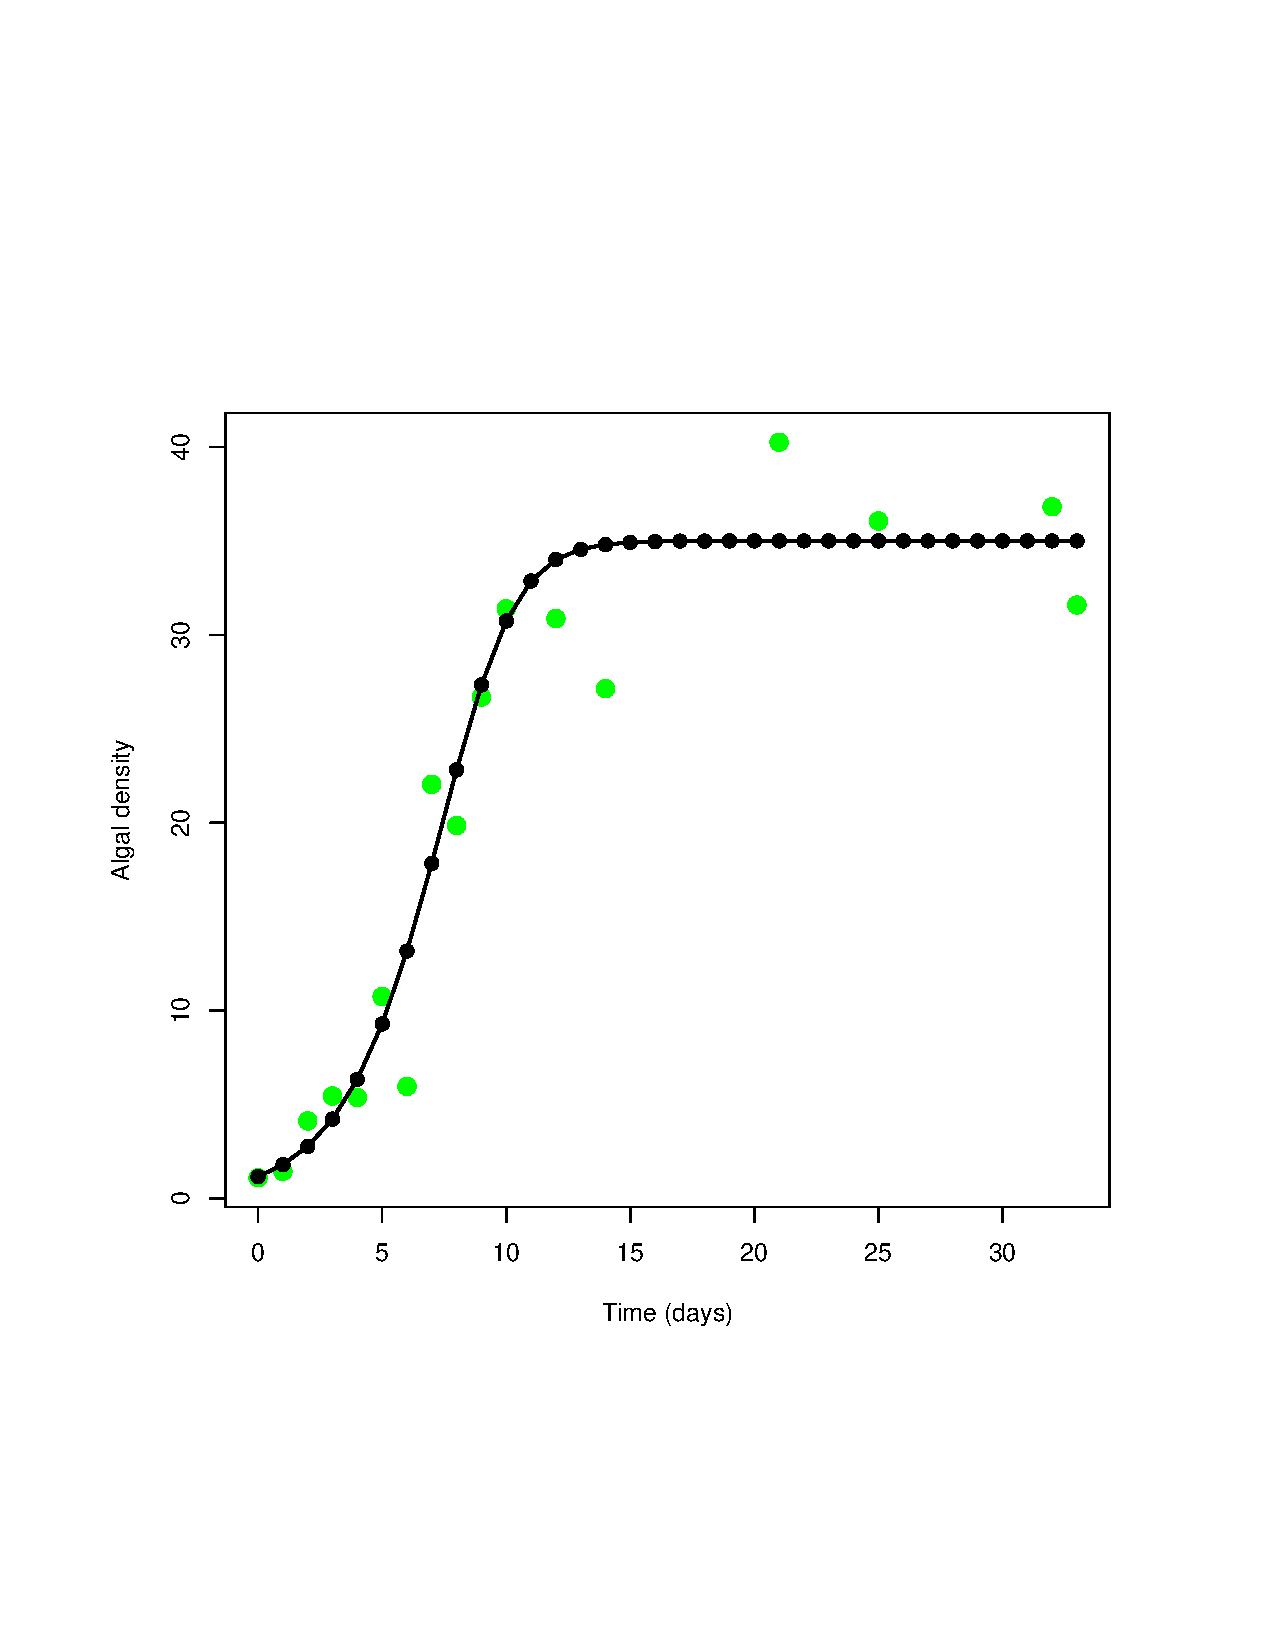
\includegraphics[width=3.5in]{figures/Session1-Fig3.pdf}}
\caption{\small{Discrete logistic model (black curve) fitted to experimental data on \textit{Chlorella} growth from
the Fussmann et al. (2000) experimental system (green points).}}
\label{Session1Fig3}
\end{figure}

Finally, we want to see how well model \eqref{dl} fits the data. To see how that
can be done, look at \textbf{Session1.3.R}. The first sections are familiar:
reading in the data and finding the parameter values. Then comes something
new: a ``for-loop'' to solve the model by stepping forward one day at a time,
starting from our estimated value at $t=0$.
We'll learn about this later -- for now, just take it for granted: 
\blst
xvals=numeric(34); xvals[1]=x0; 
for(j in 2:34) {xvals[j]=R*xvals[j-1]*(1-b*xvals[j-1])}
\end{lstlisting} 
The part to notice now is how to put the data and model solutions onto the
same plot:
\blst
plot(tvals,cvals,type="p",pch=16,cex=1.5, col="green",xlab="Time (days)",
     ylab="Algal density"); 
points(0:33,xvals,type="o",pch=16,cex=1,col="black",lwd=2); 
\end{lstlisting} 
The \texttt{plot} command is familiar with one new wrinkle: the ``col'' variable sets the 
plotting color. The \ttt{points} function is just like \ttt{plot} except that 
it adds new points (or lines) to the most recent plot, rather than making a new plot. 

\textbf{Important NOTE:} it is good practice to start each script by 
clearing R's memory of variables that were created by earlier work, as follows: 
\blst
  rm(list=ls(all=TRUE)); # clear past actions from R's memory 
\end{lstlisting}   
This avoids a lot of headaches. A script might run because a variable that it needs was 
created earlier (not within the current script), and it holds values unrelated to your current work. 
The script will then run, without any error messages, but the results will be garbage. And, when  
the TA runs your script, that variable doesn't exist so the script will not run. 
\textit{You do not want this to happen.} Make sure that \emph{every} 
script starts with clearing the memory, and that the same is true for 
\emph{every} exercise if you do several exercises in one script. The best approach is
to have a separate file for each exercise; and before you turn it in, close R, restart R, and
see if your script runs in a ``clean'' workspace. 
    
\textbf{Exercise\exnumber} The axes in plots are scaled automatically, but sometimes
you want to control them yourself, for example you may want several graphs with exactly the
same axes limits. You can control scaling using the \texttt{xlim} and \texttt{ylim}
arguments in \texttt{plot}: the general syntax is \\ 
\hspace*{1in}  \texttt{plot(x,y,xlim=c(x1,x2), ylim=c(y1,y2)) } \\
For example,  
\\ 
\hspace*{1in}  \texttt{plot(x,y,type="l",xlab="x",ylab="y",xlim=c(1,5), ylim=c(.2,1)) } \\
will draw a graph with the x-axis going from 1 to 5, the y-axis from 0.2 to 1.0.  
The file \textbf{ChlorellaGrowth.txt} has data on the maximum algal growth rate $r_{max}$ as a function of light intensity
$L$. Write a script that loads these data into \R, and 
creates a plot of growth rate versus light intensity with the
x axis running from 0 to 120, and the y axis running from 1 to 4. Save this
script for use in the next exercise. $\maltese$ 

\textbf{Exercise\exnumber} Several separate graphs can be placed  
within a single figure by using the \texttt{par} 
function (short for ``parameter'') to adjust the layout of the plot. For example the 
command \\
\hspace*{0.5in} \texttt{par(mfrow=c(m,n))} \\
divides the plotting area into $m$ rows and $n$ columns. Then as a series of \texttt{plot}
commands are used to draw graphs, successive graphs are placed along the top row from left to right, 
then along the next row, and so on.
\ttt{mfcol=c(m,n)} has the same effect except that successive graphs are placed
down the first column, then down the second column, and so on. \texttt{par} can't be
put inside of a \texttt{plot()} command -- it has to be separate and it has to come
before the plots are drawn. 

Save a copy of your script from the last exercise under a new name, and modify it as follows. 
Use \texttt{mfcol=c(2,1)} to create graphs of (1) growth rate as a 
function of Light, and (2) log(growth rate) as a function of log(Light), within one figure.  
Do the same again, using \texttt{mfcol=c(1,2)}. $\maltese$ 

\textbf{Exercise\exnumber} Use \texttt{?par} to read about other plot control parameters
that can be set using \texttt{par()}. Then write a script that draws a $2 \times 2$ set of plots,
each showing the line $y=5x+3$ with $x$ running from 3 to 8, but with 4 different
line styles and 4 different line colors. (Note: setting x=3:8 and y=5*x+3 will create
a set of x and y values to draw the line that you need). $\maltese$ 

\textbf{Exercise\exnumber} Modify one of your scripts so that
at the very end it saves the plot to disk. In Windows, this can
be done using \ttt{savePlot}; for other OS's, you can use \ttt{dev.print}.
Use the Help system to find out about these functions (e.g., \ttt{?savePlot}). 
Note that the argument \texttt{filename} in \ttt{savePlot}, and the argument
\ttt{file} in \ttt{dev.print}, can include the 
path to a folder, for example in Windows you can use \\
\hspace*{0.5in} \ttt{filename="c:/temp/MyFigure2".} \\ $\maltese$ 

\textbf{Note:} These are really exercises in using the Help system, with 
the bonus that you learn about \texttt{plot}. (Let's see, 
we know \texttt{plot} can graph data points...maybe it can also draw a 
line to connect the points, or just draw the line and leave out the points. 
That would be useful. So let's try \texttt{?plot} and see if it says anything 
about lines...Hey, it also says that \texttt{graphical parameters can be given 
as arguments to plot}, so maybe I can set line colors inside the plot command 
instead of using \texttt{par} all the time....). The Help system is 
\textit{very} helpful once you get used to it. 

\section{Vectors} 
In R, vectors and matrices are just 1- and 2-dimensional rectangular arrays of 
numbers. Operations with vectors and matrices may seem a bit abstract now, but we need them to do 
useful things later. 

We've already seen two ways to create vectors in \R: \\
1. A command in the console window or a script file listing the values, 
such as \\
\hspace*{1in} \texttt{> initialsize=c(1,3,5,7,9,11)}.\\
2. Using \texttt{read.table()}, for example: \\  
\hspace*{1in} \verb! initialsize=read.table("c:\\temp\\initialdata.txt")! \\ (Note: if the file you're trying to load doesn't exist, this is not
going to work!).  

Once it has been created, a vector can be used in calculations as if it were a number (more or less) 
\blst
> finalsize=initialsize+1; newsize=sqrt(initialsize); finalsize; newsize; 
[1]  2  4  6  8 10 12
[1] 1.000000 1.732051 2.236068 2.645751 3.000000 3.316625
\end{lstlisting}

Notice that the operations were applied to every entry in the vector. 
Similarly, commands like \texttt{initialsize-5, 2*initialsize, initialsize/10} 
apply subtraction, multiplication, and division to each element of the 
vector. The same is true for exponentiation, 
\blst
> initialsize^2;
[1]   1   9  25  49  81 121
\end{lstlisting}

In \R the default is to apply functions and operations to vectors
in an \textit{element by element} manner; anything else (e.g. matrix
multiplication) is done using special notation (discussed below). 
\textbf{NOTE}: this is the \textit{opposite} of \textsc{Matlab},
where matrix operations are the default and element-by-element requires
special notation. 

\subsection*{Functions for vector construction}
Some of the main functions for creating and working with vectors are
listed in Table \ref{VectorFunctions}. 
A set of regularly spaced values can be constructed with the \texttt{seq}
function, whose syntax is \\
\hspace*{1in} \texttt{seq(from,to,by)} or \texttt{seq(from,to,length)} \\
The first form generates a vector \texttt{(from,from+by,from+2*by,...)}
with the last entry not being larger than \texttt{to}. If a value for
\ttt{by} is not specified, its value is assumed to be 1 or -1, depending on
whether \texttt{from} or \texttt{to} is larger. The second generates a vector
of \ttt{length} evenly-spaced values, running from \ttt{from} to \ttt{to}, for
example 
\blst
> seq(1,3,length=6)
[1] 1.0 1.4 1.8 2.2 2.6 3.0
\end{lstlisting}
There are also two shortcuts for creating vectors with \texttt{by=1}:
\blst
> 1:8; c(1:8);
[1] 1 2 3 4 5 6 7 8
[1] 1 2 3 4 5 6 7 8
\end{lstlisting}

A constant vector such as \texttt{(1,1,1,1)} can be created with \texttt{rep}
function, whose basic syntax is \verb! rep(values,lengths)!. For example,
\blst
> rep(3,5)
[1] 3 3 3 3 3 
\end{lstlisting}
created a vector in which the value 3 was repeated 5 times. \ttt{rep}
can also be used with a vector of values and their associated lengths, for example
\blst
> rep( c(3,4),c(2,5) )
[1] 3 3 4 4 4 4 4
\end{lstlisting}
The value 3 was repeated 2 times, followed by the value 4 repeated 5 times.

\begin{table}[b]
\begin{tabular}
{p{110pt}p{320pt}}
\hline 
\hline 
\texttt{seq(from,to,by=1)} & Vector of evenly spaced values with specified increment (default = 1) \\
\ttt{seq(from,to,length)} & Vector of evenly spaced values with specified length \\
\texttt{c(u,v,...) } & Combine a set of numbers and/or vectors into a single vector \\
\texttt{rep(a,b)} & Create vector by repeating elements of \ttt{a} by amounts in \ttt{b} \\
\texttt{hist(v)} & Histogram plot of value in v \\
\texttt{mean(v),var(v),sd(v)} & Population mean, variance, standard deviation estimated from values in \ttt{v} \\
\texttt{length(v)} & Length of vector \texttt{v}  \\
\texttt{cor(v,w)} & Correlation between two vectors \\
\hline
\end{tabular}
\caption{\small{Some important R functions for creating and working with vectors. Many of these have other optional
arguments; use the help system (e.g. \ttt{?cor}) for more information. Note that statistical functions such as
\texttt{var} regard the values as samples from a population (rather than a list of value for the entire
population) and compute an estimate of the population statistic; for example \ttt{sd(1:3)=1}.}}
\label{VectorFunctions}
\end{table}

\R also has many functions for creating vectors of random numbers 
with various distributions, that are useful in simulating stochastic
models. Most of these have a number of \textbf{optional arguments}, 
which means in practice that you can choose to specify their value, or
if you don't a default value is assumed. For example, \ttt{x=rnorm(100)}
generates 100 random numbers with a Normal (Gaussian) distribution having mean=0, standard
deviation=1. But \ttt{rnorm(100,2,5)} 
yields 100 random numbers from a Gaussian distribution with mean=2, standard deviation=5.

Here, and in the \R documentation and help pages, the existence of default values for 
some arguments of a function is indicated 
by writing (for example) \textbf{rnorm(n, mean=0, sd=1)}. Since no default value is given for $n$, 
the user must supply one: \texttt{rnorm()} gives an error message. 

Some of the functions for creating vectors of random numbers are listed
in Table \ref{RNGs}. Functions to evaluate the corresponding distribution functions
are also available. For a listing use the Help system: ?Normal, ?Uniform, ?Lognormal,
etc. will list and explain the available functions for each distribution family. 

\begin{table}[t]
\begin{tabular}
{p{120pt}p{310pt}}
\hline
\hline 
\texttt{rnorm(n,mean=1,sd=1)} & Gaussian distribution(mean=mu, standard deviation=sd) \\
\texttt{runif(n,min=0,max=1)} & Uniform distribution on the interval (min,max) \\
\texttt{rbinom(n,size,prob)} & Binomial distribution with parameters \ttt{size}=\#trials $N$, 
\ttt{prob}=probability of success $p$ \\
\texttt{rpois(n,lambda)} & Poisson distribution with mean=lambda \\
\texttt{rbeta(n,shape1,shape2)} & Beta distribution on the interval $[0,1]$ with shape parameters 
shape1, shape2 \\
\hline
\end{tabular}
\caption{\small{Some of the main \R function for generating vectors of $n$ random numbers. To create random 
matrices, these vectors can be reshaped using the \ttt{matrix()} function, for example: \ttt{matrix(rnorm(50*20),50,20)} 
generates a $50 \times 20$ matrix of Gaussian(0,1) random numbers.}}
\label{RNGs}
\end{table}

\textbf{Exercise\exnumber} Create a vector \texttt{v=(1 5 9 13)} using \texttt{seq}.  
Create a vector going from 1 to 5 in increments of 0.2 first by using  \texttt{seq},
and then by using a command of the form \texttt{v=1+b*c(i:j)}. $\maltese$ 

\textbf{Exercise\exnumber} Generate a vector of 5000 random numbers from a Gaussian distribution
with mean=3, standard deviation=2. Use the functions \texttt{mean, sd} to compute
the sample mean and standard deviation of the values in the vector, and \texttt{hist}
to visualize the distribution. $\maltese$ 

\textbf{Exercise\exnumber} The sum of the geometric series $1 + r + r^2 + r^3 + ... + r^n$ 
approaches the limit $1/(1-r)$ for $r < 1$ as $n \rightarrow \infty$.   
Write a script that computes the sum for $r=0.5$ and $n=10$, and write a script that computes the sum. 
Compare the sum of this vector to the limiting value $1/(1-r)$. Repeat this for  
$n=50$. HINT: look at what \verb! v = c(0:5); 2^v; ! produces, and figure out why. $\maltese$ 

\subsection*{Vector addressing} 
Often it is necessary to extract a specific 
entry or other part of a vector. This is done using subscripts, for example
\blst
> q=c(1,3,5,7,9,11); q[3]
[1] 5
\end{lstlisting}
\texttt{q[3]} extracts the third element in the vector \texttt{q}. 
You can also access a block of elements using the functions for 
vector construction, e.g. 
\blst
v=q[2:5]; v
[1] 3 5 7 9
\end{lstlisting}
This has extracted 2$^{nd}$ through 5$^{th}$ elements in the vector. 
If you enter \texttt{v=q[seq(1,5,2)]}, what will happen? Try it
and see, and make sure you understand what happened. 

Extracted parts of a vector don't have to be regularly spaced. For example
\blst
> v=q[c(1,2,5)]; v
[1] 1 3 9
\end{lstlisting}

Addressing is also used to \textbf{set specific values within a vector}. For 
example, 
\blst
> q[1]=12
\end{lstlisting}
changes the value of the first entry in \texttt{q} while leaving 
all the rest alone, and 
\blst
> q[c(1,3,5)]=c(22,33,44)
\end{lstlisting}
changes the 1$^{st}$, 3$^{rd}$, and 5$^{th}$ values.  

\textbf{Exercise\exnumber}write a \textbf{one-line} command to extract 
a vector consisting of the second, first, and third elements of \texttt{q} 
\textbf{in that order}. $\maltese$ 

\textbf{Exercise\exnumber} Write a script file that computes values 
of $z=\frac{(x-1)}{(x+1)}$ and $w=\frac{sin(x^2)}{x^2}$ for 
$x=1,2,3,\cdots,12$ and plots both of these as a function of 
$x$ with the points connected by a line. $\maltese$ 

\subsection*{Vector orientation}
You may be wondering if vectors in \R 
are row vectors or column vectors (if you don't know what those are,
don't worry: we'll get to it later). The answer is ``both and neither''.
Vectors are printed out as row vectors, but if you use a vector in 
an operation that succeeds or fails depending on the vector's orientation, 
\R \textit{will assume that you want the operation to succeed and will proceed as 
if the vector has the necessary orientation.} For example, \R will let
you add a vector of length 5 to a $5 \times 1$ matrix or to a 
$1 \times 5$ matrix, in either case yielding a matrix of the 
same dimensions. The fact that \R wants you to succeed is both good and
bad -- good when it saves you needless worry about details, bad when it masks an error that you would rather know about. 

\section{Matrices}
A matrix is a two-dimensional array of numbers. 
Like vectors, matrices can be created by reading in 
values from a data file, using the \texttt{read.table} function.
Matrices of numbers can also be entered by creating a vector of the matrix 
entries, and then reshaping them to the desired number of rows
and columns using the \texttt{matrix} function. For example 
\blst
> X=matrix(c(1,2,3,4,5,6),2,3)
\end{lstlisting}
takes the values 1 to 6 and reshapes them into a 2 by 3 matrix. 
\blst
> X
     [,1] [,2] [,3]
[1,]    1    3    5
[2,]    2    4    6
\end{lstlisting}
Note that values in the data vector are put into the matrix 
column-wise, by default. You can change this by using the optional
parameter {\tt byrow}). For example 
\blst
> A=matrix(1:9,3,3,byrow=T); A
     [,1] [,2] [,3]
[1,]    1    2    3
[2,]    4    5    6
[3,]    7    8    9
\end{lstlisting}
\R will re-cycle through entries in the data vector, if need be,
to fill out a matrix of the specified size. So for example 
\texttt{matrix(1,50,50)} creates a $50 \times 50$ matrix of all 1's.

\textbf{Exercise\exnumber} Use a command of the form \texttt{X=matrix(v,2,4)}
where v is a data vector, to create the following matrix X
\blst
     [,1] [,2] [,3] [,4]
[1,]    1    1    1    1
[2,]    2    2    2    2
\end{lstlisting} 

\textbf{Exercise\exnumber} Use \texttt{rnorm} and \texttt{matrix} to 
create a $5 \times 7$ matrix of Gaussian random numbers with
mean 1 and standard deviation 2. 
 
Another useful function for creating matrices is \texttt{diag}.
\texttt{diag(v,n)} creates an $n \times n$ matrix with data
vector $v$ on its diagonal. So for example \texttt{diag(1,5)}
creates the $5 \times 5$ \textit{identity matrix}, which has 1's on
the diagonal and 0 everywhere else.

Finally, one can use the \ttt{data.entry} function. 
This function can only edit existing matrices, but for example \\
\hspace*{1in} \ttt{A=matrix(0,3,4); data.entry(A)} \\
will create \ttt{A} as a $3 \times 4$ matrix, and then call up 
a spreadsheet-like interface in which the values can be changed to
whatever you need.  

\begin{table}[t]
\begin{tabular}{p{128pt}p{300pt}}
\hline
{\tt matrix(v,m,n)} & $m \times n$ matrix using the values in v \\
{\tt data.entry(A)} & call up a spreadsheet-like interface to edit the values in A \\
{\tt cbind(a,b,c,...)} & combine compatible objects by binding them along columns \\
{\tt rbind(a,b,c,...)} & combine compatible objects by binding them along rows \\
{\tt outer(v,w)} & ``outer product'' of vectors \ttt{v,w}: the matrix whose $(i,j)^{th}$
element is \ttt{v[i]*w[j]} \\
{\tt diag(n)} & $n \times n$ identity matrix \\
{\tt diag(v)} & diagonal matrix with vector \texttt{v} on the diagonal \\
{\tt dim(X)} & dimensions of matrix X. \ttt{dim(X)[1]}=\#rows, \ttt{dim(X)[2]}=\#columns \\
{\tt rowSums(X),colSums(X)} & sum of each row or column of matrix X  \\
{\tt rowMeans(X),colMeans(X)} & mean of each row or column of matrix X  \\
{\tt apply(A,MARGIN,FUN)} & apply the function \ttt{FUN} to each row of A (if MARGIN=1) or each 
column of A (if MARGIN=2). See ?apply for details and examples. \\
\hline
\end{tabular}
\caption{Some important functions for creating and working with matrices. Many
of these have additional optional arguments; use the Help system for full details.}
\label{MatrixFunctions}
\end{table}

\subsection{cbind and rbind} 
If their sizes match, vectors can be combined to form matrices, and matrices
can be combined with vectors or matrices to form other matrices. The functions
that do this are \textbf{cbind} and \textbf{rbind}. 

\texttt{cbind} binds together columns of two objects. One thing it can do
is put vectors together to form a matrix: 
\blst
> A=cbind(1:3,4:6,7:9); A
     [,1] [,2] [,3]
[1,]    1    4    7
[2,]    2    5    8
[3,]    3    6    9
\end{lstlisting}
Remember that \R interprets vectors as row or column vectors according to
what you're doing with them. Here it treats them as column vectors so that 
columns exist to be bound together. On the other hand, 
\blst
>  B=rbind(1:3,4:6); B
     [,1] [,2] [,3]
[1,]    1    2    3
[2,]    4    5    6
\end{lstlisting}
treats them as rows. Now we have two matrices that can be combined. 

\textbf{Exercise\exnumber} Verify that \texttt{rbind(A,B)} works,  \texttt{cbind(A,A)}
works, but \texttt{cbind(A,B)} doesn't. Why not? $\maltese$ 

\subsection{Matrix addressing}
Matrix addressing works like vector addressing except that you have 
to specify both the row and column, or range of rows and columns. For 
example \texttt{q=A[2,3]} sets q equal to 8, which is the (2$^{nd}$ row, 
3$^{rd}$ column) entry of the matrix \textbf{A} , and 
\blst
> A[2,2:3]; 
[1] 5 8
> B=A[2:3,1:2]; B
     [,1] [,2]
[1,]    2    5
[2,]    3    6
\end{lstlisting} 
There is an easy shortcut to extract entire rows or columns: leave out the limits. 
\blst
> first.row=A[1,]; first.row
[1] 1 4 7
> second.column=A[,2]; second.column;
[1] 4 5 6
\end{lstlisting}
As with vectors, addressing works in reverse to assign values to matrix 
entries. For example,
\blst
A[1,1]=12; A
     [,1] [,2] [,3]
[1,]   12    4    7
[2,]    2    5    8
[3,]    3    6    9
\end{lstlisting}
The same can be done with blocks, rows, or columns, for example
\blst
> A[1,]=runif(3); A
        [,1]     [,2]       [,3]
[1,] 0.985304 0.743916 0.00378729
[2,] 2.000000 5.000000 8.00000000
[3,] 3.000000 6.000000 9.00000000

\end{lstlisting}

\textbf{Exercise\exnumber} Use \textbf{runif} to construct a 5$\times $5 
matrix $\B$ of random numbers with a uniform distribution between 0 and 1. (a) Extract 
from it the second row, the second column, and the 3$\times $3 matrix of the 
values that are not at the margins (i.e. not in the first or last row, or 
first or last column). (b) Use \texttt{seq} to replace the values in the first row of $\B$ by 
\texttt{2 5 8 11 14}. $\maltese$ 

\subsection{Matrix operations and matrix-vector multiplication} 
A numerical function applied to a matrix acts element-by-element. 
\blst
> A=matrix(c(1,4,9,16),2,2); A; sqrt(A);
     [,1] [,2]
[1,]    1    9
[2,]    4   16
     [,1] [,2]
[1,]    1    3
[2,]    2    4
\end{lstlisting}

The same is true for scalar multiplication and division. \textbf{Try}
2*A, A/3 \textbf{and see what you get.}

If two matrices (or two vectors) are the same size, then you can do element-by-element 
addition, subtraction, multiplication, division, and exponentiation:  
(\texttt{A+B, A-B, A*B, A/B, A\ B)}. Matrix $\times$ matrix and matrix $\times$ vector 
multiplication (when they are of compatible dimensions) is indicated by the special notation 
\texttt{\%*\%}. Remember, \textbf{element-by-element is the default in R}. This requires
some attention, because \R's eagerness to make things work can sometimes let errors get
by without warning. So for example
\blst
v=1:2; A*v
     [,1] [,2]
[1,]    1    9
[2,]    8   32
\end{lstlisting}
$A$ is a $2 \times 2$ matrix, and $v$ is a vector of size 2,
so the matrix-vector product $Av$ is legitimate. However, $Av$ should be a vector,
not a matrix. Since you (incorrectly) ``asked'' for element-by-element multiplication,
that's what \R did, ``recycling'' through the elements of v when it ran out of entries
in v before it ran out of entries in A. What you should have done is
\blst
> A%*%v
     [,1]
[1,]   19
[2,]   36
\end{lstlisting}

\section{Iteration (``Looping")}
\subsection{For-loops}
Loops make it easy to do the same operation over and over again, for 
example: 
\begin{itemize}
\item Making population forecasts 1 year ahead, then 2 years ahead, then 3, etc.
\item Updating the state of every neuron in a model network based on the inputs it 
received in the last time interval. 
\item Simulating a biochemical reaction network multiple times with different values
for one of the parameters.
\end{itemize} 

There are two kinds of loops in \R: \textbf{for} loops, and 
\textbf{while} loops. A \textbf{for} loop runs for a specified number of 
steps. These are written as 
\blst
for (var in seq) {
      commands
      }
\end{lstlisting}
Here's an example (in \textbf{Loop1.R}): 
\blst
# initial population size
initsize=4; 

# create vector to hold results and store initial size 
popsize=rep(0,10); popsize[1]=initsize;

# calculate population size at times 2 through 10, write to Command Window
for (j in 2:10) { 
      popsize[j]=2*popsize[j-1];
      x=log(popsize[j]);
      cat(j,x,"\n");
}
plot(1:10,popsize,type="l"); 
\end{lstlisting}

The first time through the loop, $j$=2. The line \verb! popsize[j]=2*popsize[j-1];! 
then does \verb! popsize[2]=2*popsize[1]! so that the solution at time 2 is calculated
from the solution at time 1. The second time through the loop, 
second time through, $j$=3, so the solution at time 3 is calculated from the
solution at time 2. This continues for $j=4,5,6,\cdots,10$, and then the loop is
finished \R moves on to executing any 
commands that occur after the end of the loop. The result that the vector \texttt{popsize} holds
the values of population size in generations 2 through 10. 

Note also the \texttt{cat} function (short for ``concatenate'')
for printing results to the console window. \texttt{cat} converts 
its arguments to character strings, concatenates them, and then prints them. 
The \verb! "\n" ! argument is a line-feed character
so that each ($j,x$) pair is put on a separate line. 

Several \texttt{for} loops can be nested within each other, which is needed 
for working with matrices as in the example below. It is important to notice 
that the second loop is \textbf{completely }within the first. Loops must be 
either \textbf{nested} (one completely inside the other) or 
\textbf{sequential} (one starts after the previous one ends). 
\blst
A=matrix(0,3,3);                  (1)
for (row in 1:3) {                (2) 
      for (col in 1:3) {          (3) 
          A[row,col]=row*col      (4)
      }                           (5)
}                                 (6)
A;                                (7) 
\end{lstlisting} 

Type this into a script file and run it; the result should be
\blst
     [,1] [,2] [,3]
[1,]    1    2    3
[2,]    2    4    6
[3,]    3    6    9
\end{lstlisting}

Line 1 creates A as a matrix of all zeros - this is an easy way to create a 
matrix of whatever size you need, which can then be filled in with 
meaningful values as your program runs. Then two nested loops are 
used to fill in the entries. Line 2 starts a loop over the rows of A, and 
immediately in line 3 a loop over the columns is started. To 
fill in the matrix we need to consider all possible values for the pair 
(row, col). So for row=1, we need to consider col=1,2,3. Then for 
row=2 we also need to consider col=1,2,3, and the same for row=3. That's 
what the nested for-loops accomplish. For row=1 (as requested in line 2), 
the loop in lines 3-5 is executed until it ends. Then we get to the end in 
line 6, at which point the loop in line 2 moves on to row=2, and so on.

Nested loops also let us automate the process of running a simulation many
times, for example with different parameters or to look at the average over
many runs of a stochastic model. For example (\textbf{Loop2.R}), 
\blst
p=rep(0,5);                         (1) 
for (init in c(1,5,9)){             (2) 
      p[1]=init;                    (3) 
      for (j in 2:5) {              (4) 	
         p[j]=2*p[j-1]              (5) 
         cat(init,j,p[j],"\n");     (6) 	  
      }                             (7) 
}                                   (8) 
\end{lstlisting}

Line 1 creates the vector p.
Line 2 starts a loop over initial population sizes
Lines 4-7 does one ``population growth'' simulation
Line 8 then closes the loop over initial sizes

The result when you run \textbf{Loop2.R} is that the ``population growth" 
calculation is done repeatedly, for a series of values of the initial 
population size. To make the output a bit nicer we can add some headings
as the program runs - run \textbf{Loop3.R} and then look at the file 
to see how the formatting was done. 

If this discussion of looping doesn't make sense to you, \textbf{stop now  
and get help}. Loops are essential from here on out. 

\textbf{Exercise\exnumber:} Imagine that while doing fieldwork in some 
distant land you and your assistant have picked up a parasite that grows 
exponentially until treated. Your case is more severe than your assistant's: 
on return to Ithaca there are 400 of them in you, and only 120 in your 
assistant. However, your field-hardened immune system is more effective. In 
your body the number of parasites grows by 10 percent each day, while in 
your assistant's it increases by 20 percent each day. That is, for you  
$n(j+1) = 1.1 n(j)$ starting from $n=400$ on day 1, while for your assistant
$m(j+1) = 1.2 m(j)$ starting from $m=120$ on day 1. 

Write a script file that uses a for-loop to compute the 
number of parasites in your body and your assistant's over the next 30 days, 
and draws a single plot of both on log-scale (i.e. $log(n(j))$ and $log(m(j))$ versus 
time for 30 days). The function \texttt{matplot} is useful for putting both $n$ and $m$ on 
one graph. Save a copy of the script, with the name \textbf{Parasite1.R}, for use in
future exercises. 

NOTE: this can be done without loops, but for the sake of learning, use a for-loop to 
sequentially compute $n(j)$ and $m(j)$ for $j=2$ to 31.  $\maltese$ 

\textbf{Exercise\exnumber:} Write a script file that uses for-loops to create the 
following 5$\times $5 matrix A. \underline{Think first:} do you want to use
nested loops, or sequential? 
\[
{\begin{array}{*{20}c}
 0 \hfill & 1 \hfill & 2 \hfill & 3 \hfill & 4 \hfill \\
 {0.1} \hfill & 0 \hfill & 0 \hfill & 0 \hfill & 0 \hfill \\
 0 \hfill & {0.2} \hfill & 0 \hfill & 0 \hfill & 0 \hfill \\
 0 \hfill & 0 \hfill & {0.3} \hfill & 0 \hfill & 0 \hfill \\
 0 \hfill & 0 \hfill & 0 \hfill & {0.4} \hfill & 0 \hfill \\
\end{array} }
\] $\maltese$ 

\textbf{Exercise\exnumber} Write a script file that uses a for-loop to calculate 
solutions of the difference equation model 
$$N(j + 1) = 2e^{-0.2j}N(j)/(1 + N(j)), \quad N(1) = 1$$
up to $j=13$. Remember that in \R, $e^x$ is computed using the \ttt{exp} function. Then, have your script plot $N(j)$ versus time $j$ using \texttt{type="b"} in \texttt{plot}, so that $N(t)$ is plotted as points connected by lines.  $\maltese$ 

\section{Branching}
\subsection{if-else blocks}
Sometimes the rules for ``what happens next'' in a model need 
to depend on the current values of state variables. The \textbf{if} 
statement lets us do this; the basic format is 
\blst
if(condition) {
    some commands
}else{
    some other commands
}
\end{lstlisting}
An  \texttt{if} block can be set up in other ways, but the layout 
above, with the \}else\{ line to separate the two
sets of commands, can always be used. 

If the ``else" is to do nothing, you can leave it out:
\blst
if(condition) {
    commands
}
\end{lstlisting}

\begin{table} [t!]
\begin{tabular}{p{120pt}p{200pt}}
\hline
x $<$ y  & less than	\\
x $>$ y  & greater than \\
x $<=$ y & less than or equal to \\
x $>=$ y & greater than or equal to \\
x $==$ y & equal to \\
\hline 
\end{tabular}
\caption{Some comparison operators in \R. Use ?Comparison to learn more.}
\label{Comparisons}
\end{table}

The conditions controlling a \textbf{while} loop are built up from operators 
that compare two variables (Table \ref{Comparisons}). 
These operators return a logical value of TRUE or FALSE. For example, 
try:  
\blst
> a=1; b=3; c=a<b; d=(a>b); c; d;
\end{lstlisting}
The parentheses around (a$>$b) are optional but can be used to improve 
readability in script files. 

When we compare two vectors or matrices of the same size, or compare a 
number with a vector or matrix, comparisons are done element-by-element.  
For example,
\blst
> x=1:5; b=(x<=3); b
[1]  TRUE  TRUE  TRUE FALSE FALSE
\end{lstlisting}

\R also does arithmetic on logical values, treating TRUE as 1 and 
FALSE as 0. So \verb! sum(b) ! returns the value 3, telling us that 3 
entries of x satisfied the condition (x$<=$3). This is useful for
running multiple simulations and seeing how often one outcome
occurred rather than another. 

\textbf{Exercise\exnumber} Look at and source \textbf{a copy of} \textbf{Branch1.R} to 
see an \texttt{if} statement which makes the population growth rate depend on the 
current population size. $\maltese$ 

More complicated decisions can be built up by nesting
one \texttt{if} block within another, i.e. the ``other commands''
under \texttt{else} can include a second \texttt{if} block.   
\textbf{Branch2.R }uses this method to have population growth tail off 
in several steps as the population size increases: 

\blst
for (i in 1:50) {                    (1)
    if(popnow<250){                  (2)
        popnow=popnow*2;             (3)
    }else{                           (4) 
        if(popnow<500){              (5)
            popnow=popnow*1.5        (6)
        }else{                       (7)
            popnow=popnow*0.95       (8)
        }                            (9) 
    }                                (10)
    popsize=c(popsize,popnow);       (11)
}                                    (12)
\end{lstlisting}

What does this accomplish? \begin{itemize}
\item If \texttt{popnow} is still $<250$, then 
line 3 is executed growth by a factor of 2 occurs. Since the \texttt{if} condition was 
satisfied, the entire \texttt{else} block (line numbers 5-10 above)
isn't looked at; \R jumps line (11) and continues from there. 

\item If popnow is not $<250$, \R moves 
on to the \texttt{else} on line 4, and immediately encounters the \texttt{if} 
on line 5. 

\item If popnow is $<500$ the growth factor of 1.5 
applies, and \R then jumps to the \textbf{end} and continues from there. 

\item If neither of the two \texttt{if} conditions is satisfied, the 
final \texttt{else} block is executed and population declines by 
5{\%} instead of growing. 
\end{itemize} 

\textbf{Exercise\exnumber} Starting from a copy of your script \textbf{Parasite1.R}, modify the 
script so that there is random variation in parasite success, depending on whether
or not conditions on a given day are stressful. Specifically, on ``bad days'' the parasites increase
by 10\% while on ``good days'' they are beaten down by your immune system and they go 
down by 10\%, and similarly for your assistant. Specifically, 
\begin{equation*}
\begin{aligned}
\mbox{If day \emph{j} is bad:  }  & n(j+1)=1.1 \times n(j), & \mbox{ and } m(j+1)=1.2\times m(j) \hfill \\
\mbox{If day \emph{j} is good: }  & n(j+1)=0.9\times n(j), & \mbox{ and } m(j+1)=0.8\times m(j) \hfill \\
\end{aligned}
\end{equation*} 
Do this by using \texttt{runif(1)} and an \texttt{if} statement
to one ``toss a coin'' for each day: if the random value produced by \texttt{runif} for
that day is $<0.5$ it's a good day, and otherwise it's bad. Make sure that your script does a new 
``coin toss'' for each day, but that the same toss applies to both you and your assistant.   $\maltese$ 

\subsection{While-loops [advanced]} 
A \texttt{ while} loop lets an iteration continue until 
some condition is satisfied. For example, we can solve a model until some 
variable reaches a threshold. The format is
\blst
while(condition){
      commands
}
\end{lstlisting}

The loop repeats as long as the condition remains true. \textbf{Loop4.R} 
contains an example similar to the for-loop example; source it to get a 
graph of population sizes over time. A few things to notice about the program: 
\begin{enumerate}
\item Although the condition in the while loop said \texttt{while(popsize<1000)}
the last population value was $>1000$. That's because the loop condition is 
checked \textbf{before} the commands in the loop are executed. When the 
population size was 640 in generation 6, the condition was satisfied so the 
commands were executed again. After that the population size is 1280, so the 
loop is finished and the program moves on to statements following the loop. 
\item Since we don't know in advance how many iterations are needed, we 
couldn't create in advance a vector to hold all the results. Instead, a vector 
of results was constructed by starting with the initial population size and 
appending each new value as it is calculated. . 
\item When the loop ends and we want to plot the results, the ``y-values'' are 
popsize, and the x values need to be 0:something. To find ``something'', the 
\texttt{length} function is used to find the length of popsize.  
\end{enumerate}
 
Within a while-loop it is often helpful to have a \textbf{counter} variable
that keeps track of how many times the loop has been executed. 
In the following code, the counter variable is \texttt{n}: 
\blst
n=1; 
while(condition) {
    commands
    n=n+1; 	
}
\end{lstlisting}
The result is that \texttt{n=1} is true while the \texttt{commands} (whatever they are)
are being executed for the first time. Afterward \texttt{n} is set to 2, and this remains
true during the second time that the commands are executed, and so on. One use of counters
is to store a series of results in a vector or matrix: on the $n^{th}$
time through the commands, put the results in the $n^{th}$ entry of the vector, $n^{th}$ row
of the matrix, etc.  

\textbf{Exercise\exnumber} Write a script file that uses 
a while-loop to compute the number of parasites in your body and your 
assistant's so long as you are sicker than your assistant (i.e. so long as 
$n>m$) and stops when your assistant is sicker than you. Use a copy of the
originail, unmodified \textbf{Parasite1.R} as your starting point. $\maltese$ 


\subsection{Logical operators [advanced]} 

More complicated conditions in if-else structures and while loops can be built by using \textbf{logical operators} to 
combine comparisons: 
\blst
!              Negation 
& &&           AND 
| ||           OR 
\end{lstlisting}
OR is \textbf{non-exclusive}, meaning that \texttt{x|y} is true 
if x is true, if y is true, or if both x and y are true. 
For example: \\
\texttt{>> a=c(1,2,3,4); b=c(1,1,5,5); (a<b){\&}(a>3); (a<b)$\vert $(a>3);}

An alternative to \verb! (x==y) ! is the \texttt{identical} function.  
\texttt{identical(x,y)} returns TRUE if x and y are exactly the same, 
else FALSE. The difference between these is that if (for example) 
x and y are vectors (x==y) will return a vector of values for
element-by-element comparisons, while \texttt{identical(x,y)}
returns a single value: TRUE if each entry in x equals the
corresponding entry in y, otherwise FALSE. You can use ?Logical to
read more about logical operators. 

\textbf{Exercise\exnumber} Use the \texttt{identical} function to construct
a one-line command that returns TRUE if each entry in a vector
\texttt{rnorm(5)} is positive, and otherwise returns FALSE. 
\textbf{Hint:} \texttt{rep} works on logical variables, so \texttt{rep(TRUE,5)} 
returns the vector \texttt{(TRUE,TRUE,TRUE,TRUE,TRUE)}. $\maltese$ 



\section{Numerical Matrix Algebra} \label{MatComp}
\R has functions for matrix-algebra calculations that use ``industry standard'' 
numerical libraries (LINPACK, EISPACK, BLAS, LAPACK) libraries. Some of these functions are listed in 
Table \ref{LinAlgFunctions}. 

\begin{table}[t]
\begin{tabular}{p{120pt}p{300pt}}
\hline
{\tt eigen(A)} & eigenvalues and eigenvectors \\
{\tt t(A)} & transpose of A \\
{\tt solve(A)} & inverse of matrix A \\
{\tt solve(A,B)} & solution $x$ of the linear system $Ax=b$ for each column $b$ of the matrix $B$\\
{\tt det(A)} & determinant of the matrix A \\
{\tt norm(A)} & matrix norm of A (several options)\\
{\tt exp(A)} & matrix exponential $\exp(A)=\sum\limits_{n \geqslant 0}\frac{A^n}{n!}$ (in package \ttt{fMultiVar}) \\ 
{\tt mtx.exp(A,n)} & efficiently compute powers of a matrix $A^n$ (not element-by-element) (in package \ttt{BioDem}) \\
{\tt apply(A,margin,fun)} & apply a function \ttt{fun} to the rows (margin=1) or columns (margin=2) of matrix A,
and return all resulting values \\
{\tt sapply(v,fun)} & apply a function \ttt{fun} to all elements in vector v, returning a vector of values \\
\hline
\end{tabular}
\caption{Some important functions for matrix algebra calculations. Many
of these have additional optional arguments; use the Help system for full details.}
\label{LinAlgFunctions}
\end{table}


Some of \R's matrix functions only work on square matrices and will return an error if 
\textbf{A} is not square, in particular functions for computing eigenvalues and
eivenvectors. \textit{For the remainder of this section we only 
consider square matrices}. 

\subsection{Eigenvalues and eigenvectors}
Because eigenvalues are so important for studying dynamic models, we will now 
study \texttt{eigen} in some detail. Recall that if $Aw=\lambda w$ (for $A$ a square matrix,
$w$ a nonzero column vector, and $\lambda$ a real or complex number) then $\lambda$
is called an \textit{eigenvalue} and $w$ is the corresponding \textit{eigenvector} of $A$. 
If $v$ is a row-vector such that $vA= \lambda v$, then $v$ is called a \textit{left
eigenvector} of A. The left eigenvalues for a matrix are the same as the (right) 
eigenvalues.

We are often most interested in the dominant eigenvalue, which depending on
context (discrete versus continuous time models) means either the one 
with the largest absolute value, or the one with the largest real 
part.\footnote{The general definition of absolute value, which covers both real and complex 
numbers, is that $\left| {a + ib} \right|$ is the positive square root of $(a^2 + b^2)$, where $i= \sqrt{-1} .$} 
In \R, the \texttt{abs} function computes the absolute value of a real or complex number 
(and acts element-by-element on vectors and matrices).

\texttt{eigen} returns eigenvalues sorted by absolute value, with the largest first. 
For example,
\blst
A=matrix(1:9,3,3); vA=eigen(A); vA;
$values
[1]  1.611684e+01 -1.116844e+00 -4.054215e-16

$vectors
           [,1]       [,2]       [,3]
[1,] -0.4645473 -0.8829060  0.4082483
[2,] -0.5707955 -0.2395204 -0.8164966
[3,] -0.6770438  0.4038651  0.4082483
\end{lstlisting}
As with the output from \ttt{lm} in our first interactive
session (you remember \ttt{lm} \ldots) vA is a compound \emph{object} composed of
two \emph{components}, whose names are \texttt{values}
and \texttt{vectors}. The ``\$'' is used to extract components
of a compound object. For example \texttt{vA\$values} is the
\texttt{values} part of \texttt{vA}, a vector consisting of the sorted eigenvalues: 
\blst
vA$values
[1] 1.611684e+01 -1.116844e+00 -4.054215e-16
\end{lstlisting} 
As noted above, \ttt{va\$values[1]} is the eigenvalue with 
the largest absolute value.   

The \ttt{vectors} component is a matrix whose columns are the corresponding
eigenvectors, sorted in the same order as the eigenvalues. That is, 
\blst
j=1; A%*%vA$vectors[,j]-vA$values[j]*vA$vectors[,j];
              [,1]
[1,]  0.000000e+00
[2,] -3.552714e-15
[3,] -3.552714e-15
\end{lstlisting}
This calculation verifies the definition of eigenvalues and eigenvectors: $A v_1 = \lambda_1 v_1$,
so $A \vec v_1 -\lambda_1 \vec v_1 = \vec 0$. The [2,] and [3,] values above are really zeros, but because eigenvalues and eigenvectorsare computed numerically, there is a small amount of numerical error. 

\textbf{Exercise\exnumber} Verify that the output is also $(0,0,0)$, apart
from numerical error, for j=2 and j=3. Explain in words what these
calculations show. $\maltese$ 

\textbf{Exercise\exnumber} Enter the command \ttt{names(vA)} and
see what results. From this, infer what the \ttt{names} function does. 
Enter the command \ttt{names(A)} and infer the meaning of the 
object \texttt{NULL} in \R. Check your guess by using the Help
menu on the console window: select \textsf{R language (standard)} 
and type \textsf{NULL} into the popup window that appears.  $\maltese$ 

To get the left eigenvectors of a matrix, we use the fact that 
the left eigenvectors of a matrix A are the eigenvectors of its transpose, \ttt{t(A)}. So \\
\hspace*{1in} \ttt{vLA=eigen(t(A))\$vectors} \\
gets you the left eigenvectors of A.  

\textbf{Exercise\exnumber} Compute \texttt{vLA[,j]\%*\%A-vA\$values[j]*vLA[,j]}
to verify the last claim about left eigenvectors, for j=1 to 3. $\maltese$ 

\textbf{Eigenvector scalings: } For a transition matrix model, the dominant right 
eigenvector $w$ (i.e. the eigenvector corresponding to the eigenvalue with largest absolute value)
is the \emph{stable stage distribution}, so we are most interested in relative 
proportions. To get those, \ttt{w=w/sum(w)}. The dominant left eigenvector \textbf{v} is 
the reproductive value, and it is conventional to scale those relative to the 
reproductive value of a newborn. If newborns are class 1: \ttt{v=v/v[1]}. 

\textbf{Exercise\exnumber}: Write a script file which applies the above to 
the matrices 
\[
A = \left( {\begin{array}{*{20}c}
   1 & { - 5} & 0  \\
   6 & 4 & 0  \\
   0 & 0 & 2  \\
 \end{array} } \right)\quad B = \left( {\begin{array}{*{20}c}
   0 & 1 & 5  \\
   0.6 & 0 & 0  \\
   0 & 0.4 & 0.9  \\
 \end{array} } \right)
\]
finding \textbf{all} the eigenvalues and then extracting the dominant one and the 
corresponding left and right eigenvectors. For $B$, use the scalings 
defined above.  $\maltese$ 

\subsection{Eigenvalue sensitivities and elasticities}
For an $n \times n$ matrix \textbf{A} with entries $a_{ij}$, the sensitivities 
$s_{ij} $and elasticities $e_{ij} $can be computed as

\begin{equation}
s_{ij} = \frac{\partial \lambda }{\partial a_{ij} } = \frac{v_i w_j 
}{\left\langle {v,w} \right\rangle }\quad \quad e_{ij} = \frac{a_{ij} 
}{\lambda }s_{ij} 
\label{SensitivityFormula}
\end{equation}

\noindent
where $\lambda$ is the dominant eigenvalue, \textbf{v} and \textbf{w} are 
dominant left and right eigenvectors, and $\left\langle {v,w} \right\rangle $ 
is the inner product of \textbf{v} and \textbf{w}, computed in \R as 
\texttt{sum(v*w).} So once $\lambda $, \textbf{v}, and \textbf{w} have been 
found and stored as variables, it just takes some for-loops to compute the 
sensitivies and elasticities.
\blst
vA=eigen(A); lambda=vA$values[1];
w=vA$vectors[,1]; w=w/sum(w); 
v=eigen(t(A))$vectors[,1]; v=v/v[1];
vdotw=sum(v*w); 
s=A; n=dim(A)[1]; 
for(i in 1:n) {
    for(j in 1:n) {
        s[i,j]=v[i]*w[j]/vdotw;
    }
}
e=(s*A)/lambda; 
\end{lstlisting}

Note how all the elasticities are computed at once in the last line. 
In \R that kind of ``vectorized" calculation is \emph{much} quicker than 
computing entries one-by-one in a loop. Even better is to use a built-in function 
that operates at the vector
or matrix level. In this case we can use \ttt{outer} to completely 
eliminate the nested do-loops: 
\blst
vA=eigen(A); lambda=vA$values[1];
w=vA$vectors[,1]; w=w/sum(w); 
v=eigen(t(A))$vectors[,1]; v=v/v[1];
s=outer(v,w)/sum(v*w); 
e=(s*A)/lambda; 
\end{lstlisting}

Vectorizing code to avoid or minimize loops is an important
aspect of efficient \R programming. 

\textbf{Exercise\exnumber} Construct the transition matrix \textbf{A}, 
and then find $\lambda $, \textbf{v}, \textbf{w} for an age-structured model 
with the following survival and fecundity parameters. Then use those to construct
the elasticity matrix for \textbf{A}. 

Ages 0-5 are genuine ages with survival probabilities
$(p_0, p_1, \cdots, p_5 ) = (0.3, 0.4, 0.5, 0.6, 0.6, 0.7)$

Note that $p_j = a_{j + 1,j}$, the chance of surviving from age $j$ to age 
$j+1$, for these ages. You can create a vector \ttt{p} with the 
values above and then use a for-loop to put those values into 
the right places in \ttt{A}. 

Age 6 (or older) are adults with survival 0.9 and fecundity 12. 
\[
A = \left( {\begin{array}{*{20}c}
   0 & 0 & 0 & 0 & 0 & 0 & {12}  \\
   {.3} & 0 & 0 & 0 & 0 & 0 & 0  \\
   0 & {.4} & 0 & 0 & 0 & 0 & 0  \\
   0 & 0 & {.5} & 0 & 0 & 0 & 0  \\
   0 & 0 & 0 & {.6} & 0 & 0 & 0  \\
   0 & 0 & 0 & 0 & {.6} & 0 & 0  \\
   0 & 0 & 0 & 0 & 0 & {.7} & {.9}  \\

 \end{array} } \right)
\] $\maltese$ 

\textbf{Results (with some rounding)}:\\
$\lambda =1.042$ \\
$w = (0.6303,0.1815,0.0697,0.0334,0.0193,0.0111,0.055)$ \\
$v = (1,3.47,9.05,18.85,32.73,56.83,84.59)$ \\


\textbf{Exercise\exnumber} For the projection matrix 
\blst
 A = matrix(c(
   0.44,   6.0,   67.4,  183.1,
   0.0048, 0.44,  3.04,  8.3,
   0,      0.21,  0.042, 0.083,
   0,     0.0089, 0.031, 0.014),4,4,byrow=TRUE); 
\end{lstlisting}
use the \textbf{which} function with \texttt{arr.ind=TRUE} to find all
entries of the elasticity matrix for A that are above the average of the
positive entries of the elasticity matrix. HINT: see
what \texttt{A[A>0]} returns, and use that construction in computing the
average of the positive entries.  $\maltese$ 


\subsection{Finding the eigenvalue with largest real part [advanced]}
For the Jacobian matrix of a differential equation model, the dominant eigenvalue is the one with the 
largest real part. To find this, and the associated
eigenvector, we need to extract the real parts of the eigenvalues and locate
the largest one. 

Use the help system -- (\ttt{?complex}) -- to see the \R functions for working
with complex numbers. The one we need now is \ttt{Re}, which extracts
the real parts of complex numbers. 

Use \ttt{data.entry} to create the matrix
\[
A = \left( {\begin{array}{*{20}c}
   3 & 0 & 0  \\
   2 & 2 & {-3}  \\
   0 & 3 & 1  \\
\end{array} } \right)
\]
and you should find that \ttt{eigen(A)\$values} are \\
\hspace*{1in} \ttt{[1] 1.5+2.95804i 1.5-2.95804i 3.0+0.00000i}. \\
The first two are a complex conjugate pair with absolute value
3.316625 (\ttt{mod(eigen(A)\$values)} gets you the absolute values of
the eigenvalues), but the third one has the largest real part. 

To have \R do this for you, we use the \ttt{which} function to find
which eigenvalue is dominant (i.e., which has the largest real part). 
Run the code below, and follow what it's doing; see \ttt{?which} and
\ttt{?max} if you need to. 
\blst
vA=eigen(A)$values;           # find the eigenvalues
rmax=max(Re(vA));             # find the largest Real part of any eigenvalue
j=which(Re(vA)==rmax);        # which eigenvalue is dominant? 
lmax=vA[j];                   # dominant eigenvalue 
vmax=eigen(A)$vectors[,j];  # dominant eigenvector 
\end{lstlisting} 

\textbf{Exercise\exnumber} Try the above on \ttt{A=diag(c(1,2,3))} and see
what you get for \ttt{j,r,lmax} and \ttt{vmax}. Try it again for 
\ttt{A=diag(c(1,2,sqrt(as.complex(-9))))} and \ttt{A=diag(c(3,1,3))}, and make
sure that you understand what happens in each case. $\maltese$ 


\section{Writing your own functions}
A lot of \R's power comes from all its built-in functions, such as \texttt{plot} and
\texttt{lm}. A function gets some information from you, and then uses it to do
something (like draw a figure) or to compute 
something (like a set of eigenvalues). 

\R also lets you write your own functions, which then 
act like built-in functions (except that they go away when you close an R session). 
Sometimes this is just a convenience. Using functions makes it easier to see the 
logical flow of a large program. But sometimes functions are essential, 
such as when you want to solve a set of 
differential equations.  

\R code for defining a function has a very specific structure, but it can go anywhere
in a script file. It goes like this example:
\blst 
plotLine=function(x,y) {
    plot(x,y,type="p",cex=1.5)
    fit = lm(y~x)
    abline(fit,col="red")
}	
\end{lstlisting} 

\begin{figure}[tbp]
\centerline{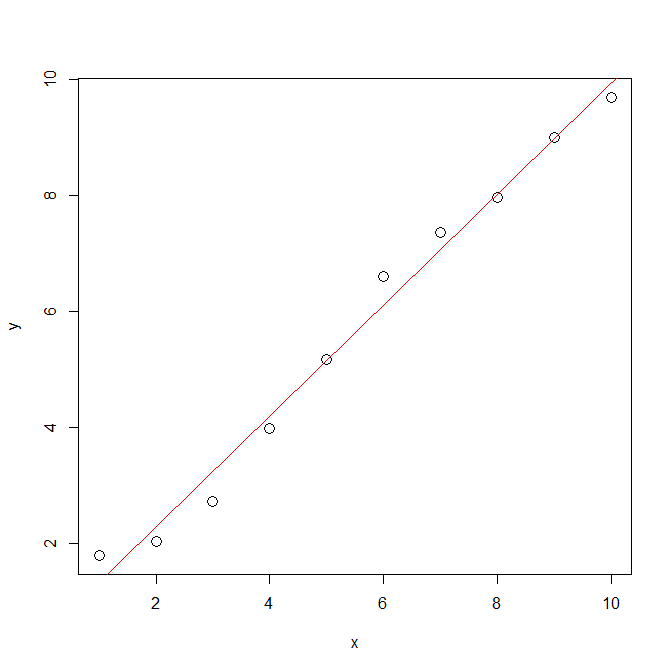
\includegraphics[width=2.5in]{figures/plotLine.png}}
\caption{Figure produced by the \texttt{plotLine} function}
\label{fig:plotLine}
\end{figure} 

The first line of code specifies the name of the function, \texttt{plotLine}, and its \emph{arguments}: the 
information it is going to work with (in this case, numeric vectors \texttt{x} and \texttt{y} of the same length). 
In between the \{ and the \} are the \R commands that the function will carry out. To see what
this function accomplishes, do the following Exercise right now. It should create a plot like Figure
\ref{fig:plotLine}. 

\textbf{Exercise \exnumber} Open up a new empty script file, copy-paste the code above into your script, 
and run the script. Then go into the \R console window and enter the following code:
\vspace{-0.2in}
\blst
  x = 1:10
  y = x+0.5*rnorm(10)
  plotLine(x,y)
\end{lstlisting} 
\vspace{-0.2in} 

$\maltese$  

Functions can also be written so that they return things that they calculated, like the 
\texttt{eigen} function does. Here is an example: 
\blst 
plotLine2=function(x,y) {
    plot(x,y,type="p",cex=1.5)
    fit = lm(y ~ x)
    abline(fit,col="red")
    return(fit$coef)
}	
\end{lstlisting} 
Again, copy-paste this code into a script, run the script, and then in the \R console window, enter
\blst
pars = plotLine2(x,y)
pars
\end{lstlisting} 
You should see that the \tw{return} statement in \tw{plotLine2} resulted in the regression coefficients
(namely \tw{fit\$coef}) getting returned from the function, so that the 
command \tw{pars=plotLine2(x,y)} put the coefficients vector into the variable \tw{pars}.     

\textbf{Exercise \exnumber} Write a function \tw{whatzit=function(x,y,z)} that takes three numbers (or vectors) $x,y,z$ 
as its arguments, and returns $x+y+z$. Make sure that it works by running the function like you did with \tw{plotLine},
and then in the \R console window the command \tw{whatzit(1,2,3)} should give you 6 as the result: 
\vspace{-0.15in}
\blst 
> whatzit(1,2,3)
[1] 6
\end{lstlisting} 
\vspace{-0.2in}
$\maltese$ 

Functions can return several different values, by combining them into a 
multi-part object with named parts. For example, 
\blst 
mysquare=function(v,w) {
    q=v^2; r=w^2
    return(list(vSquared=q,wSquared=r))
}
\end{lstlisting}
You can then extract the components in the \R's usual way. 
\blst 
> x=mysquare2(1:4,2:5); names(x);
[1] "vSquared" "wSquared"
> x$vSquared
[1]  1  4  9 16
\end{lstlisting}

\textbf{Exercise\exnumber} Write a function \texttt{stats(v)} that takes as input a single
vector, and returns a list with named components \texttt{average} (mean of the values in the vector),
and \texttt{variance} (population variance estimated from the values in the vector, using \texttt{var}). 
Verify that once you've run the script with the function definition, you get 
\blst
> stats(1:21);
$average
[1] 11
$variance
[1] 38.5
\end{lstlisting} 
\vspace{-0.2in}
$\maltese$ 

\section{A simulation project}
This section is an optional ``capstone'' project putting into use the  
programming skills that have been covered so far. Nothing new about
\R \textit{per se} is covered in this section.  

The exercise is to first write, and then use, a script file that simulates a simple model for density-independent 
population growth with spatial variation. The model is as follows. The \textit{state variables}  
are the numbers of individuals in a series of $L = 20$ 
patches along a line ($L$ stands for ``length of the habitat") . 
\begin{table}[h!]
\centering
\begin{tabular}
{|p{22pt}|p{22pt}|p{22pt}|p{22pt}|p{22pt}|p{22pt}|p{22pt}|p{22pt}|p{22pt}|p{22pt}|p{22pt}|p{22pt}|}
\hline
1& 
2& 
3& 
4& 
... & 
& 
& 
& 
& 
...& 
L-1& 
L \\
\hline
\end{tabular}
\end{table}

Let $N_j(t)$ denote the number of individuals in patch $j$ ($j=1,2,\ldots, L$) at 
time $t$ ($t=1,2,3,\ldots$ ), and let $\lambda_j$ be the geometric growth rate 
in patch $j$. The \textit{dynamic equations} for this model consist of two steps:
\begin{enumerate}
\item Geometric population growth within patches: 
\begin{equation}
M_j(t) = \lambda _j N_j(t) \quad \mbox{ for all } j. 
\end{equation}
\item Dispersal of some individuals between neighboring patches:
\begin{equation}
N_j(t + 1) = (1 - 2d)M_j(t) + dM_{j - 1}(t) + dM_{j + 1}(t) \quad \mbox{ for } 2 \le j \le L-1 
\label{disperse1}
\end{equation}
where $2d$ is the ``dispersal rate". We need special rules for the end patches. 
For this exercise we assume \textit{reflecting boundaries}: those who exit  
into the void have the sense to come back. That is, there is no 
leftward dispersal out of patch 1 and no rightward dispersal out of patch $L$:
\begin{equation}
\begin{array}{l}
 N_1(t + 1) = (1 - d)M_1(t) + dM_2(t) \\ 
 N_L(t + 1) = (1 - d)M_L(t) + dM_{L - 1}(t) \\ 
\end{array}
\label{disperse2}
\end{equation}
\end{enumerate} 

\textbf{Exercise\exnumber} As a first step, write a function \texttt{reflecting} that implements the dispersal phase, equations
\ref{disperse1} and \label{disperse2}. That is, the arguments to the function are a pre-dispersal population vector \texttt{Mt} and the dispersal
parameter $d$, and the function returns the population vector after dispersal has taken place.
\blst
reflecting <- function(Mt,d) {
   ...
   ... your code to compute Nt1, the population vector N at time t+1
   ...
return(Nt1)
}
\end{lstlisting} 

This function takes a vector \texttt{Mt} of length $L$ as input, and returns a vector of equal length as output. Equation
\ref{disperse1} says that \texttt{Nt1[2:(L-1)]} is the sum of 3 terms: individuals that stay in the same patch, individuals that
come in from the left (patches 1 to $L-2$), and individuals that come in from the right (patches 3 to $L$).
Think about how you can compute each of these 3 terms without using any loops, and then add them up to
compute most values in \texttt{Nt1}. After that, you need two more lines to compute the values for patches 1 and $L$.
Note that the code in reflecting has to ``figure out'' what the value of $L$ is -- so what is the R function that
tells you the length of a vector?$\maltese$ 

\textbf{Exercise\exnumber} Using your \texttt{reflecting} function write a script
to simulate the model. \\
$\bullet$ Write your script to \underline{start} with 5 individuals in each patch at 
time $t$=1, \underline{iterate} the model up to $t$=100, and \underline{graph} 
the log of the total population size (the sum over all patches) over time. Use the 
following growth rates: $\lambda _j = 0.9$ in the left half of the patches, 
and $\lambda _j = 1.2$ in the right. \\
$\bullet$ Write your program so that $d$ and $L$ are parameters, 
in the sense that the first line of your script file reads \\
\verb!   d=0.1; L=20;! \\
and the program will still work if these are changed to other values. $\maltese$ 

Note that this model is not totally different from iterating a matrix population model, in that you start with
a founding population at time 1 (described by a vector) and use a loop to compute successive populations at
times 2,3,4, and so on. So the script can be structured like the scripts for matrix models. After you specify
the values of $d$ and $L$, and create the vector of $\lambda$ values, you should create a matrix \texttt{N} with $L$ rows and 100
columns, so that \texttt{N[j,t]} will be $N_j(t)$. The initial population goes into the first column of \texttt{N}, and the model
is simulated by doing a loop over time (denoted by k in the code below)
\blst
for(k in 2:200){ # k is the time index
   ... compute Mt from column k-1 of N, and the lambda values
   ... compute Nt1 using the reflecting function
   ... put Nt1 into N, in the right place
}
\end{lstlisting} 
As in the reflecting function, try to vectorize! Vector/matrix operations are much faster than loops. For
example, set things up so that in the for-loop, computing the entire \texttt{Mt} vector is a one-line statement of
the form \texttt{a=b*c}.

\textbf{Exercise\exnumber} Use the model (modified as necessary) to ask how the spatial 
arrangement of good versus bad habitat patches affects the  
population growth \emph{rate}. For example, does it matter if all the good sites 
($\lambda >1$) are at one end or in the middle? What if they aren't all in 
one clump, but are spread out evenly (in some sense) across the entire 
habitat? \textbf{Be a theoretician}: (a) Patterns will be easiest to see if 
good sites and bad sites are very different from each other. (b) Patterns 
will be easiest to see if you come up with a nice way to compare growth 
rates across different spatial arrangements of patches. (c) Don't confound 
the experiment by also changing the proportion of good versus bad patches, at
the same time you're changing the spatial arrangement. $\maltese$ 

\section{Coin tossing and Markov Chains} 
\label{Mchain}

The exercises on coin tossing and Markov chains in Chapter 3 of the textbook can be used
as the basis for a computer-lab session. For convenience we also 
include them here. All of the \R functions and programming methods required for these exercises 
have been covered in previous sections, but it is useful to ``remember''
\begin{itemize}
\item how to generate sets of random uniform and Gaussian random numbers using 
\texttt{runif} and \texttt{rnorm}.
\item how logical operators can be used to convert a vector of numbers into a vector of 1's and 0's 
according to whether or not a condition holds.
\item how to find the places in a vector where the value changes, using logicals
and \texttt{which}.
\end{itemize}  
\blst
>> x = rnorm(20);  
>> y = as.numeric(x<0.3); 
>> z = which(y[2:20]!=y[1:19])
\end{lstlisting}
Take a look at \texttt{x,y,z} and make sure you understand why each one is what it is. 

\subsection{Coin tossing} 

\textbf{Exercise\exnumber} Experiment with sequences of coin flips produced by a random number generator: 
\begin{itemize}
\item Generate a vector \texttt{x} of 1000 random numbers uniformly
distributed in the unit interval $[0,1]$.
\item Compute and plot a histogram for the values with 10 equal bins of length 0.1. How much variation is there 
in values of the histogram? Does the histogram make you suspicious that the numbers are not independent and 
uniformly distributed random numbers? 
\item Now compute sequences of 10000 and 100000 random numbers uniformly
distributed in the unit interval $[0,1]$, and a histogram for each with ten equal bins.
Are your results consistent with the prediction that the range of variation
between bins in the histogram is proportional to the square root of the sequence length?
\end{itemize}
Note: \ttt{q=hist(runif(1000),10)} will plot the first histogram you need, and \ttt{q\$counts} will
be a vector of the number in each bin of the histogram, so instead of eyeballing the range of
variation you can use \texttt{range} and \texttt{sd}. $\maltese$ 

The theoretical ``benchmark'' for this experiment, and its relation to coin tossing, goes as follows. 
Let $X_i$ be 1 if the $i^{th}$ random number falls into the first bin of the histogram, otherwise $X_i=0$,
for $i=1,2,3,\cdots n$. So each $X_i$ is a coin toss with $P(H)=0.1$. The fraction of tosses that fall
in the first bin is then $f=(X_1+X_2 + \cdots X_n)/n$. Using the basic properties of means and variances,
we can derive that $E(f)=E(X)$ and $Var(f)=Var(X)/n$. The 10 bins of the histogram that you constructed
can be regarded as (approximately) 10 repetitions of this experiment, because there's nothing special
about bin 1: they all have the same ``probability of Heads''. So if you compute \\
\hspace*{1.5in} \ttt{n=10000; q=hist(runif(n),10); f1=q\$counts/n; sqrt(var(f1))} \\
and then compute \ttt{f2} with $n=100,000$, you should see (what?) 

\textbf{Exercise\exnumber} (a) Recall that coin tossing is modeled by
the binomial distribution: the probability of $k$ heads in a sequence of $n$ tosses, with $p=0.6$ being
the probability of heads, is given by  
$$c_k (0.6)^k (0.4)^{1000-k} \quad \mbox{ where } c_k =
\begin{pmatrix} 1000\\ k \\ \end{pmatrix} = \frac{1000!}{k!(1000-k)!}.$$ 
In \R, the binomial coefficient $\begin{pmatrix} n\\ k\\ \end{pmatrix}$ is computed using \ttt{choose(n,k)},
e.g. \ttt{choose(1000,5)} gives $\begin{pmatrix} 1000\\ 5\\ \end{pmatrix}$. 

Calculate the probability of $k$ heads for values of $k$ between 500 and 700 in a sequence of 1000
independent tosses.  Plot your results with $k$ on the $x$-axis and the probability of $k$ heads on the $y$-axis.
Comment on the shape of the plot. 

(b) Generate a sequence of 1000 uniformly distributed random numbers \texttt{r}, as in the last
exercise, convert them into a sequence of coin tosses in which the probability of heads is $0.6$
and the probability of tails is $0.4$, and compute the total number of heads in the 1000 coin tosses. 
Write a script that does this 1000 times (i.e., 1000 repetitions
of tossing 1000 coins) and for each repetition stores (in a vector) the total number of heads. Now 
test the binomial distribution by plotting a histogram of the number of heads obtained in each repetition,
and compare the results with the predictions of the binomial distribution. 
 
(c) Modify the last experiment by doing 10000 repetitions of 100
coin tosses. Comment on the differences you observe between this
histogram and the histogram for 1000 repetitions of tossing 1000 coins. $\maltese$ 

\textbf{Tossing multi-sided coins}
Uniform random numbers can also be used to simulate ``coin-toss'' experiments where the
coin has 3 or more sides. Conceptually this is easy. If there are $n$ sides with 
probabilities $p_1,p_2,\cdots,p_n$, you generate \ttt{r=runif(1)} and declare that 
\begin{itemize}
\item[] Side 1 occurs if $r \le p_1$.
\item[] Side 2 occurs if $p_1 < r \le p_1+p_2$
\item[] Side 3 occurs if $p_1 + p_2 < r \le p_1 + p_2 + p_3$
\item[] $\cdots$
\item[] Side $n$ occurs if $p_1 + p_2 + \cdots + p_{n-1} < r.$
\end{itemize} 
To code this compactly in \R, note that the outcome depends on the cumulative sums
$$c_1=p_1, \quad c_2=p_1+p_2, \quad c_3 = p_1 + p_2 + p_3, \quad \cdots, c_n=1.$$
If $r$ is larger than exactly $k$ of these, then the outcome is Side $k+1$. Cumulative
sums of a vector are computed using the function \ttt{cumsum}. 

As an example, the following code tosses a 5-sided coin with probabilities
given by the vector \ttt{p} defined in the first line:
\blst
p=c(.3,.1,.3,.1,.2); b=cumsum(p); 
side=sum(runif(1)>b)+1 
\end{lstlisting}

To toss the coin repeatedly you can use the \ttt{sapply} function, which applies 
an arbitrary function to all elements in a vector. 
\blst
side=sapply(runif(1000),FUN=function(x) sum(x>b)+1)
\end{lstlisting} 
In the code above the function to be applied is defined within the call to \ttt{sapply}. More
complicated functions can be defined separately, prior to the call, as in the following example: 
\blst
side.choose=function(x) {sum(x>b) +1} 
side=sapply(runif(1000),FUN=side.choose)
\end{lstlisting} 

\textbf{Exercise\exnumber} Generate 10000 tosses of a 3-sided coin (with your choice
of probabilities), and plot a histogram of the results to verify that your coin is
behaving the way it should. $\maltese$ 

\subsection{Markov chains and residence times} 
The purpose of the following exercises is to generate synthetic data for 
single channel recordings from finite state Markov chains, and to explore patterns in the ``data''. 
Single channel recordings give the times that a Markov chain makes a transition from a closed to an open
state or vice versa. The histogram of expected residence times 
for each state in a Markov chain is exponential, with different mean residence time for different states.  
To observe this in the simplest case, we again consider coin tossing. The two outcomes, heads or
tails, are the different states in this case. Therefore the histogram of residence times for heads and tails should 
each be exponential. The following steps are taken to compute the residence times:
\begin{itemize}
\item Generate sequences of independent coin tosses based on given probabilities.
\item Look at the number of \emph{transitions} that occur in each of the sequences 
(a \emph{transition} is when two successive tosses give different outcomes).
\item Calculate the residence times by counting the number of tosses between each transition. 
\end{itemize}

\textbf{Exercise \exnumber} Find the script \texttt{cointoss.R}. This program calculates
the residence times of coin tosses by the above methodology, and plots the frequency distribution of residence
times in two different ways: a histogram of the number of residence times of each length, and a semi-log plot of
the frequency of residence times of each length. Are these results consistent with the prediction 
that the histograms decreases exponentially? To answer this question, write an R script to make a plot 
that compares the predicted results with the simulated residence times stored in 
the vectors \texttt{hhist} and \texttt{thist}. 

The predicted result about the histogram for H residence times comes from the following argument: 
a run of exactly $k$ H's in a row occurs whenever there is a $T$ followed by exactly $k$ H's in a row, followed 
by another T. The probability of this chain of events is $(1-p)^2 p^k$, where $p$ is the probability of getting H 
on a single toss. So how many runs of exactly $k$ H's in a row should occur in a sequence of \texttt{nt} coin tosses? 

Your script should overlay predicted values on the histograms plotted by \texttt{cointoss.R}, and on the
semi-log plots of frequences. $\maltese$ 

Models for stochastic switching among conformational states of membrane channels are more complicated than 
a series of independent coin tosses. There are usually more than 2 states, and the transition probabilities are state dependent. Moreover, in measurements some states cannot be distinguished 
from others. We can observe transitions from an open state to a closed
state and vice versa, but transitions between open states (or between closed states)
are ``invisible''. 

Here we will simulate data from a Markov chain with 3 states, and then collapse that data to remove the distinction 
between 2 of the states. We will then analyze the data, as in the previous exercise, 
to see that the residence time distributions are not consistent with a Markov chain with just two states. 
We can then use the distributions of residence times in the observations, 
to reach conclusions about how many states we actually have.

We will consider a membrane that has three states: two closed states $C_1$ and $C_2$, and one open state $O$. 
We assume that direct transitions between $C_1$ and $O$ are impossible, but that the intermediate state
$C_2$ has a shorter residence time than $C_1$ and $O$. Here is the transition
matrix of a Markov chain we will use to simulate these conditions:
\begin{eqnarray*}
&\begin{matrix}C_1&C_2&O\end{matrix}&\\
&\displaystyle{\begin{bmatrix}.98&.1&0\\
                              .02&.7&.05\\
                               0 &.2&.95\end{bmatrix}}
&\begin{matrix}C_1\\C_2\\O\end{matrix}
\end{eqnarray*}
You can see from the matrix that the probability $0.7$ of staying in
state $C_2$ is much smaller than the probability $0.98$ of staying in
state $C_1$ or the probability $0.95$ of remaining in state $O$.

\textbf{Exercise\exnumber} Generate a set of 100000 samples
from the Markov chain with these transition probabilities. We will
label the state $C_1$ by 1, the state $C_2$ by 2 and the state $O$ by 3.
This can be done by a modification of the method that we used to toss coins
with 3 or more sides. The modification is that the probabilities
of each side depend on the current state of the membrane: 
\blst
nt = 100000;
A = matrix(c(0.98, 0.10, 0, 0.02, 0.7, 0.05, 0, 0.2, 0.95),3,3,byrow=T);
B = apply(A,2,cumsum); #cumulative sums of each column 
A; B; 
states=numeric(nt+1); rd=runif(nt);  
states[1] = 3; # Start in open state
for(i in 1:nt) {
   b=B[,states[i]]; #cumulative probabilities for current state  
   states[i+1]=sum(rd[i]>b)+1 # do the ``coin toss'' based on current state 
}
plot(states[1:1000],type="s"); 
\end{lstlisting}
Notice the use of \ttt{apply} to compute the cumulative sum of each  
column of the transition matrix, and \ttt{type="s"} to get a ``stairstep''
plot of the state transitions (see \ttt{?plot}). $\maltese$ 

\textbf{Exercise\exnumber} Compute the eigenvalues and eigenvectors of
the matrix $A$. Compute the total time that your ``data'' in the 
vector \texttt{states} spends in each state (use vector operations to do this!)
and compare the results with predictions coming from the dominant right
eigenvector of $A$.  $\maltese$ 

\textbf{Exercise\exnumber} Produce a new vector \texttt{rstates} by taking the vector 
\texttt{states} that you previously generated (from a 3-state Markov chain) and ``reducing''
the data so that states 1 and 2 are indistinguishable. You can do that by 
defining \texttt{rstates=states}, changing every 2 in \texttt{rstates} to 1, 
then changing every 3 to 2. The states of \texttt{rstates} will be called ``closed'' 
(when \texttt{rstates=1})  and ``open'' (when \texttt{rstates}=2). $\maltese$ 

\textbf{Exercise\exnumber}
Plot the frequency distribution of residence times of the open and closed
states in \texttt{rstates} by applying the methods used in  
\texttt{cointoss.R}. Comment on the shapes of the distributions in each case.
Using your knowledge of the transition matrix $A$, make a prediction
about what the residence time distributions of the open states should be, and 
compare this prediction with the data. Then, show that the residence time distribution
for the closed states is not fit well by an exponential distribution.  $\maltese$ 

\section{The Hodgkin-Huxley model}
The purpose of this section is to develop an understanding of the 
components of the Hodgkin-Huxley model for the membrane potential of
a space-clamped squid giant axon. It goes with the latter part
of Chapter 3 in the textbook, and with the \textbf{Recommended reading:} 
Hille, Ion Channels of Excitable Membranes, Chapter 2.

The Hodgkin-Huxley model is the system of differential equations
\begin{equation}
\begin{aligned} 
C \frac{dv}{dt} & =i - \left[m^{3}h g_{Na}\left(v-v_{Na}\right) 
+n^{4}g_{K}\left(v-v_{K}\right) +g_{L} \left(v-v_{L}\right) \right]  \\
\frac{dm}{dt}& =3^\frac{T-6.3}{10} \left[ (1-m) \Psi\left(\frac{-v-35}{10}\right) 
-4m \exp \left(\frac{-v-60}{18}\right) \right] \\
\frac{dn}{dt}&=3^\frac{T-6.3}{10} \left[ 0.1 \left( {1-n} \right) \Psi \left(\frac{-v-50}{10} \right) 
-0.125 n \exp \left(\frac{-v-60}{80} \right) \right]  \\
\frac{dh}{dt}&=3^\frac{T-6.3}{10} \left[0.07 {\left( {1-h}\right) 
\exp \nolimits \left( {{{-v-60} \over {20}}}\right) -{{h} \over {1+ \exp \nolimits ({-0.1(v+30)})}}} \right] 
\end{aligned}
\label{HHfull} 
\end{equation}
$$ \mbox{where} \qquad \qquad \Psi(x) = \frac{x}{\exp(x) - 1}. $$
The state variables of the model are the membrane potential $v$ and the ion channel
gating variables $m$, $n$, and $h$, with time $t$ measured in msec. Parameters are 
the membrane capacitance $C$, temperature $T$, conductances $g_{Na},g_K,g_L$, 
and reversal potentials $v_{Na},v_K,v_L$. The gating variables represent channel 
opening probabilities and depend upon the membrane potential.
The parameter values used by Hodgkin and Huxley are 
\begin{table}[h!]
\label{HHparams}
\begin{center}
\begin{tabular}
{|p{30pt}|p{30pt}|p{30pt}|p{30pt}|p{30pt}|p{50pt}|p{30pt}|p{30pt}|}
\hline
$g_{Na}$& 
$g_K$& 
$g_L$& 
$v_{Na}$& 
$v_K$& 
$V_L$& 
$T$& 
$C$ \\
\hline
120& 
36& 
0.3& 
55& 
-72& 
-49.4011& 
6.3& 
1 \\
\hline
\end{tabular}
\end{center}
\end{table}

Most of the data used to derive the equations and estimate the parameter values comes
from voltage clamp experiments of the membrane, e.g Figure 2.7 of Hille.

In this set of exercises, we want to see that the model reproduces the
voltage clamp data well, and examine some of the approximations and 
limitations of the parameter estimation. Note that because $T=6.3$ in the parameter set
we are using, the prefactor $3^\frac{T-6.3}{10}$ in the equations for $m,n$ and $h$ equals 1,
and it can be omitted in all of the exercises. Also, the exercises all 
consider voltage clamp experiments in which the membrane potential
$v(t)$ is externally imposed, and is constant except for instantaneous jumps from one value
to another. So for the situation we are considering here, the model \eqref{HHfull} 
reduces to: 
\begin{equation}
\begin{aligned} 
\frac{dm}{dt}& =(1-m) \Psi\left(\frac{-v-35}{10}\right) -4m \exp \left(\frac{-v-60}{18}\right) \\
\frac{dn}{dt}&=0.1 \left( {1-n} \right) \Psi \left(\frac{-v-50}{10} \right) 
-0.125 n \exp \left(\frac{-v-60}{80} \right) \\
\frac{dh}{dt}&=0.07 {\left( {1-h}\right) 
\exp \nolimits \left( {{{-v-60} \over {20}}}\right) -{{h} \over {1+ \exp \nolimits ({-0.1(v+30)})}}} 
\end{aligned}
\label{HHreduced} 
\end{equation}
In voltage clamp, the membrane potential $v$ is held constant, so $\frac{dv}{dt} = 0$ and 
the first line of \eqref{HHfull} gives the following formula for the current:
\be
i(t) = m^3(t) h(t) g_{Na}(v-v_{Na}) + n^4(t) g_K (v-v_K) + g_L (v-v_L)
\label{HHcurrent}
\ee
When the membrane potential $v$ is constant, the equations for the gating 
variables $m,n,h$ are first order linear differential equations that can be rewritten 
in the form 
\begin{equation}
\tau_x \frac{dx}{dt} = -(x - x_{\infty}) 
\label{gating}
\end{equation} 
where $x$ is $m,n$ or $h$. The solution to equation \eqref{gating} is
\be 
x(t) = x_{\infty} + (x(0) - x_{\infty}) \exp(\frac{-t}{\tau_x}).
\label{gatingSolution}
\ee

\textit{Before you start doing these exercises}, please read the suggestions for getting started in the
following subsection. 

\textbf{Exercise\exnumber}
Re-write the differential equations for $m$, $n$, and $h$ in the form above, thereby obtaining expressions for 
$\tau_m,\tau_n,\tau_h$ and $m_{\infty},n_{\infty},h_{\infty}$ as functions of $v$. 

\textbf{Exercise\exnumber}
Write an R script that computes and plots $\tau_m,\tau_n,\tau_h$ and  
$m_{\infty},n_{\infty},h_{\infty}$ as functions of $v$, for $v$ varying from 
$-100$mV to $75$mV. You should obtain graphs that look like Figure 2.17 of Hille.

\textbf{Exercise\exnumber}
Write an R script to compute and plot as a function of time 
the current $i(t)$ obtained from voltage clamp experiments in which
the membrane is held at a potential of $v_0 = -60$mV 
and then stepped to a higher potential $v_s$ for $6$msec. (While the membrane is at its holding
potential $-60$mV, the values of $m,n,h$ approach $m_{\infty}(-60),n_{\infty}(-60),h_{\infty}(-60)$. Use these 
as the initial values $m(0),n(0),h(0)$). As in Figure 2.7 of Hille, compute the current as a function 
of time for $v_s = -30,-10,10,30,50,70,90$, and plot each of the curves of current on
the same graph. 

\textbf{Exercise\exnumber}
Separate the currents obtained from the voltage clamp experiments by plotting on separate graphs 
each of the sodium, potassium and leak currents.

\textbf{Exercise\exnumber}
Hodgkin and Huxley's 1952 papers explain their choice of the complicated 
functions in their model, but they had no computers available to analyze 
their data. In this exercise and the next, we examine procedures for 
estimating from experimental data the sodium current parameters 
$m_{\infty},h_{\infty},\tau_m, \tau_h$. However, the data that we will use
will be generated by the model itself. 

As in the previous Exercise, compute and plot the Hodgkin-Huxley sodium current 
generated by a voltage clamp experiment with a holding potential of $v0= -90$mV 
and steps to $v_s = -80,-70,-60,-50,-40,-30,-20,-10,0$. This is your ``data''.\footnote{Analyzing
data that come from a model in order to estimate parameters that you already know 
may sounds a bit crazy at first, but statisticians do this all the time and many of
them are not crazy. Before working with real data, it's a good idea to
generate artificial ``data'' from the model with known parameters, and make sure that your approach to 
fitting the model allows you to correctly recover the parameters that generated the ``data''.} 
Then using the expression $m^3 h g_{Na}(v - v_{Na})$ for the sodium current,
estimate $m_{\infty}$, $\tau_m$, $h_{\infty}$ and $\tau_h$ as functions
of voltage from this simulated data. The most commonly used methods assume 
that $\tau_m$ is much smaller than $\tau_h$, so that the activation variable
$m$ reaches its steady state before $h$ changes much. So for times just
after the step occurs, you can assume that $m$ is changing but $h$ is holding constant at its initial
value. For times long after the step (many multiples of $\tau_m$), you can assume that
$h$ is changing but $m$ is holding constant at its steady state value.  

Explain the procedures that you used. 
Some of the parameters are difficult to determine, especially over certain
ranges of membrane potential. Why? How do your estimates 
compare with the values computed in Exercise 12.1?

\textbf{Exercise\exnumber Challenge:} For the parameters that you had 
difficulty estimating in the previous exercise, design and simulate voltage clamp protocols
that help you estimate these parameters better. (See Hille, pp. 44-45.)
Describe your protocols and how you estimate the parameters.  
Plot the currents produced by the model for your 
new experiments, and give the parameter estimates
that you obtain using the additional ``data'' from your experiments.
Further investigation of these procedures is a good topic for a    
course project. 

\subsection{Getting started}
We offer here some suggestions for completing the exercises in this section. 

\textbf{Exercise 12.1} Complicated expressions are often built by composing simpler expressions.
In any programming language, it helps to introduce intermediate 
variables. Here, let's look at the gating variable $h$ first.
We have 
$$\frac{dh}{dt}=  0.07 \exp \left( \frac{-v-60}{20}\right )(1-h) - \frac{h}{1+\exp(-0.1(v+30)}$$
Introduce the intermediate expressions 
$$a_h = 0.07 \exp \left( \frac{-v-60}{20}\right )$$
and 
$$ b_h = \frac{1}{1+\exp(-0.1(v+30)}$$
Then 
$$\frac{dh}{dt}= a_h(1-h) - b_h h = a_h - (a_h+b_h) h$$
We can then divide this equation by $ (a_h+b_h)$ to obtain the desired form
$$\tau_h \frac{dh}{dt} = -(h - h_{\infty})$$
as 
$$\frac{1}{a_h+b_h}\frac{dh}{dt}= \frac{a_h}{a_h+b_h} - h.$$
Comparing these two expressions we have 
$$\tau_h = \frac{1}{a_h+b_h}, \qquad h_{\infty} = \frac{a_h}{a_h+b_h}.$$
We can implement this in \R to compute the values of $h_{\infty}(-45)$ and
$\tau_h(-45)$ as follows: 
\blst
v = -45;
ah = 0.07*exp((-v-60)/20);
bh = 1/(1+exp(-0.1*(v+30)));
tauh = 1/(ah+bh);
hinf = ah/(ah+bh);
\end{lstlisting}
Evaluation of this script gives tauh = 4.6406 and hinf = 0.1534.

\textbf{Exercise 12.2} To do the second exercise, you could use for-loops to compute
$\tau_m, \tau_h$, etc. at a set of $v$ values running from -100 to 75. But a better
approach is to write a set of \R functions \texttt{tau.m,tau.h}, etc., that can take as
input a vector of $v$ values, and return a vector of function values, e.g.
\blst
tau.m=function(v) {
    <stuff>
    return(something)
}
\end{lstlisting} 
Having done that, you can then make a plot of $\tau_m(v)$ with
\blst
    v=seq(-100,75,by=1)
    plot(v,tau.m(v),type="l")
\end{lstlisting}
To put several curves on the same plot, you can \texttt{cbind} them into a matrix
and use matplot:
\blst
    v=seq(-100,75,by=1)
    M=cbind(tau.m(v),tau.h(v))
    matplot(v,M,type="l")
\end{lstlisting}

For $m_\infty,\tau_m,n_\infty,\tau_n$ there is an added twist: 
the formula for the function $\Psi$ gives the  
{\it indeterminate} value $0/0$ when $x=0$, so \R cannot evaluate
it there. Nonetheless, using {\it l'Hopital's rule} from calculus, we can
define $\Psi(0) = 1$ to make $\Psi$ a smooth function. So the \textit{very first}
thing you should do is write a function to evaluate $\Psi(x)$, using 
\texttt{ifelse} to set $\Psi=1$ when $x=0$ and $x/(e^x-1)$ when $x \ne 0$.  
The \textit{very next} thing you should do, is use your function to plot 
$\Psi(x)$ over a range of values including 0, to make sure that it's working
properly. Whenever you write a function, take a minute to test it and make
sure that it's doing what it's supposed to. 

\textbf{Exercises 12.3,12.4}. To compute currents for the rest of the exercises,
it is again helpful to begin by writing functions \texttt{mvt,nvt,hvt} that
evaluate the gating variables $m,n,h$ as functions of time, $v_0$, and $v_s$ (the
holding and step-up potentials). Equation \eqref{gatingSolution}
says that, for example, 
\be
m(t)=m_{\infty}(v_s) + (m_{\infty}(v_0)-m_{\infty}(v_s))\exp(-t/\tau_m(v_s)), \qquad t \ge 0. 
\ee
and your \texttt{mvt=function(times,v0,vs)} needs to evaluate this formula. 
Once these functions have been defined, you can use them to write functions 
\texttt{i.Na,i.K,i.leak} for the individual currents, and then use those functions 
to write a function for the total current. Breaking up the computation of total 
current into a series of small pieces increases your odds of success, and leaves you with code 
that's easier to debug, understand and use.  

\textbf{Exercise 12.5} The last exercises require much more ingenuity than the previous ones. 
To get started, repeat computations like those of Exercise 12.4 to generate the sodium 
current ``data'' used in the exercise. For this exercise we assume that $v_{Na}$ is known,
so the current can be divided by $(v-v_{Na})$ to obtain the conductance $g_{Na}m^3 h$. 
As your first step, create a matrix in which each column holds the conductance values
for one value of $v_s$ at a series of closely-spaced times from $t=0$ to $t=6$ msec,
and plot those conductance curves so you can see what your ``data'' look like.   

After this is done, strategies must be developed to estimate 
$m_\infty,h_\infty,\tau_m,\tau_h$. Frequently used procedures 
assume that 
\begin{enumerate}
\item the experiment starts at a potential sufficiently hyperpolarized that there is
no inactivation (i.e. $h=1$) and 
\item activation is so fast relative to inactivation that $m$ reaches its steady state before $h$ has changed 
significantly. 
\end{enumerate}
This separation of time scales -- $m$ changing much faster than $h$ because $\tau_m \ll \tau_h$  
-- means that early, rapid changes in conductance are caused by changes in $m$, while later, slower 
changes in conductance are caused by changes in $h$. One can then estimate $m_\infty$ and $\tau_m$ from the increasing 
portion of the conductance traces, assuming that $h=1$ during this entire period
of time, so that the conductance is $g_{Na}m^3$. Under this assumption, what does the maximum value
of the conductance (at a given $v_s$) tell you about the parameters affecting $m(t)$? 

Then to estimate $\tau_h$, we assume that the decreasing ``tail'' of the conductance curve 
is given by $g_{Na}m_{\infty}^3 h(t)$, because $m(t)$ has converged to its steady state. 
The rate at which this curve converges to its limiting value $g_{Na}m_{\infty}^3 h_{\infty}$
provides an estimate of $\tau_h$. 

It is easier to estimate $h_{\infty}$ from a different set of voltage traces, having   
different values of the holding potential $v_0$, followed by a step to 
a step-up potential $v_s$ that is the same for each trace. 
In this protocol we start with $h$ partially inactivated (i.e. $h<1$), so the peak 
conductance during the subsequent trace is proportional to the initial value of $h$, which is 
$h_{\infty}(v_0).$ A plot of peak conductance as a function of $v_0$ is then \textit{proportional to} a plot
of $h_{\infty}$ as a function of $v_0$. The constant of proportionality can be inferred from
the fact that the maximum value of $h_{\infty}(v)$ is 1. Consult Hille for further 
descriptions of these protocols.

\section{Solving systems of differential equations} 
Built-in \R functions make it relatively easy to do some  
complicated things. One important example is finding numerical solutions
for a system of differential equations $$\frac{dx}{dt}=f(t,x).$$ 
Here $x$ is a vector assembled from quantities that change with time,
and the \textit{vector field} $f$ gives their rates of change. The Hodgkin-Huxley model from the
last section is one example. Here we start with the simple model of a gene regulation network 
from Gardner et al. (2000) that is described in the textbook. The model is 
\begin{equation}
\begin{split}
\frac{du}{dt} & =  -u + \frac{\alpha_u}{1+v^\beta} \\
\frac{dv}{dt} & =  -v + \frac{\alpha_v}{1+u^\gamma}
\end{split}
\label{ts_eqn}
\end{equation}
The variables $u,v$ in this system are functions of time. They
represent the concentrations of two repressor proteins $P_u, P_v$ in
bacteria that have been infected with a plasmid containing genes that
code for $P_u$ and $P_v$. The plasmid also contains promoters, with $P_u$ a
repressor of the promoter of the gene coding for $P_v$ and vice-versa.

The equations are a simple compartment model describing the 
rates at which $u$ and $v$ change with time. $P_u$ degrades at rate $1$ (so the
loss rate is $-1 \times u$) and it is 
produced at a rate $\dfrac{\alpha_u}{1+v^\beta}$, which is a decreasing
function of $v$. The exponent $\beta$ models the \textit{cooperativity} in
the repression of $P_u$ synthesis by $P_v$. The processes of
degradation and synthesis combine to give the equation for $\dfrac{du}{dt}$, and 
the equation for $\dfrac{dv}{dt}$ is similar.

There are no explicit formulas to solve this pair of equations, but we can
interpret what the equations mean geometrically. At each point of the
$(u,v)$ plane, we regard $ (\frac{du}{dt},\frac{dv}{dt})$ as a {\bf
vector} that gives the direction and magnitude for how fast $(u,v)$
jointly change as a function of $t$. Solutions to the equations give
rise to parametric curves $(u(t),v(t))$ whose tangent vectors $
(\frac{du}{dt},\frac{dv}{dt})$ are those specified by the equations.

To plot the vector field, first run the script DMBpplane.R (this script
is based on pplane.R by Daniel Kaplan, Department of Mathematics, Macalester College, and
has been modified and used here with his permission). This script includes a function
that computes the vector field for model \eqref{ts_eqn} with the assumption
that $\alpha_u=\alpha_v$: 
\blst 
toggle=function(u,v,parms) {
    du= -u + parms[1]/(1+v^parms[2]);
    dv= -v + parms[1]/(1+u^parms[3]);
    return(c(du,dv)); 
}
\end{lstlisting} 
Note how this function is set up: 
\begin{itemize}
\item Its input arguments are the two state variables \ttt{u,v} and a parameter vector \ttt{parms}. 
Even if \ttt{parms} is not used by the function, it must be included in the list of arguments 
(you can set \ttt{parms=0}).  
\item The function returns the vector field \textit{as a vector}. 
\item The computations are set up so they will go through if \ttt{u} and \ttt{v} are
matrices of equal size. This eliminates the needs for for-loops in many of the computations
that we will use to study vector fields.  
\end{itemize}
Use this setup for any vector field that you want to study using the functions in DMBpplane.R.  

The function \texttt{phasearrows} (also in DMBpplane.R) can then be used to plot the 
vector field, as in this example: 
\blst
phasearrows(fun=toggle,xlim=c(0,3),ylim=c(0,3),resol=25,parms=c(3,2,2))
\end{lstlisting}
In this statement, \ttt{fun} is the name of the function that calculates the vector field,
\ttt{xlim} and \ttt{ylim} define the range of values for the plot, and setting \ttt{resol=25}
means that arrows showing the vector field will be drawn at a $25 \times 25$ grid of points 
within the plotting region. The parameter vector \ttt{parms} is passed to the vector field
function -- this argument can be omitted if the vector field function does not use \ttt{parms}.

\textbf{Exercise \exnumber} Run DMBpplane.R to create the \ttt{toggle} function, and then 
use the command above to plot the vector field. $\maltese$ 

We can think of solutions to \eqref{ts_eqn} as curves in the plane that ``follow the arrows''. 
Given a starting point $(u_0,v_0)$, the mathematical theory discussed in the textbook proves that there 
is a unique solution $(u(t),v(t))$ with $(u(0),v(0))=(u_0,v_0)$. The process
of finding the solution numerically is called \textit{numerical integration}. Methods for
numerical integration build up an approximate solution by adding short segments of an approximate
solution curve, one after another. 

\R's numerical ODE solvers are in the \textbf{deSolve} package. Download this (if necessary) from
CRAN, and then use the command \ttt{library(deSolve)} to load it into your \R session.   

{\bf Exercise \exnumber} After you load the \textbf{deSolve} package, use \ttt{?rk4} to look at the 
syntax for this function.  $\maltese$ 

To use \R's ODE solvers, the first step is to write a function to evaluate 
the vector field \textit{in the specific format required by the solvers}. Here's what that looks like
for the toggle switch model:
\blst
Toggle=function(t,y,parms) {
    u=y[1]; v=y[2];
    du= -u + parms[1]/(1+v^parms[2]);
    dv= -v + parms[1]/(1+u^parms[3]);
    dY=c(du,dv); 
    return(list(dY)); 
}
\end{lstlisting} 
There's a bit to digest in that. Here are the things to note:
\begin{enumerate}
\vspace*{-0.12in}
\item The function \underline{must} have input arguments \ttt{(t,y,parms)}, even if only the state
vector \ttt{y} is used to compute the vector field. Here \ttt{t} is time, \ttt{y} is the state vector,
and \item \ttt{parms} is again a vector of parameter values for the function. This allows you to
see how solutions change as parameters are varied, without having to re-write and re-run the function. It also simplifies
the process of fitting differential equations to data. 
\item The vector field value has to be returned \underline{as a list}, which is why we need both
\textit{toggle} and \textit{Toggle}. There's a good reason for this;
if you're curious and have \textit{way} too much free time on your hands, \ttt{?lsoda} gives  
the explanation. You've been warned.  
\end{enumerate} 

The ``basic'' ODE solver in \R is \textbf{rk4}, which implements the 4th-order Runge
Kutta method with a fixed time step. The format is 
\blst 
out=rk4(x0,times,func,parms) 
\end{lstlisting}
Here \ttt{times} is a vector of the times at which you want solution values, 
\ttt{x0} is the value of the state vector at the initial time (i.e. \ttt{times[1]}), 
\ttt{func} func is the function specifying the model (such as \ttt{Toggle}),
and \ttt{parms} is the vector of parameter values that will be passed to func. 

Here is an example using our \ttt{Toggle} function:
\blst
x0=c(.2,.1); times=seq(0,50,by=0.2); parms=c(3,2,2);
out=rk4(x0,times,Toggle,parms)
matplot(out[,1],out[,2:3],type="l",ylim=c(0,3),xlab="time t",ylab="u,v"); 
\end{lstlisting}

{\bf Exercise \exnumber} Write a script toggle.R with the commands above, and run them
to see some solution trajectories as a function of time. Which plotted curve is
$u$, and which is $v$? How do you know? Look at the matrix \ttt{out}
to see how it is set up: the first column is a list of times, and the other columns are
the computed (approximate) values of the state variables at each time. $\maltese$ 

The state trajectories both seem to be approaching constants. 
A second way of looking at the
trajectories (\textbf{Exercise:} do this yourself right now) is: 
\blst
plot(out[,2],out[,3],type="l",xlab="u",ylab="v") 
\end{lstlisting}
This kind of plot is called a {\it phase portrait}. It shows the path in the 
$(u,v)$ {\it phase plane} taken by the trajectory, but we lose track of the 
times at which the trajectory passes through each point on this path.

\textbf{Exercise \exnumber} Use \ttt{rk4} again with initial conditions
$(0.2,0.3)$ to produce a new output matrix \ttt{out2} and plot phase portraits 
of both solutions. Do this first for time interval $[0,50]$ and again for $[0,200]$.

The trajectories appear to end at the same places, indicating that they didn't
go anywhere after $t = 50$. We can explain this by observing that the differential
equations vanish at these endpoints. The curves where $\frac{du}{dt} = 0$
and $\frac{dv}{dt} = 0$ are called \textit{nullclines} for the vector field.
They intersect at \emph{equilibrium points}, where both  $\frac{du}{dt} = 0$ 
and  $\frac{dv}{dt} = 0$. The solution with initial point an equilibrium is
constant. Here, the equilibrium points are \emph{(asymptotically) stable}, meaning
that trajectories close to the equilibria approach them as $t$ increases. $\maltese$ 

Nullclines for a general vector field can be plotted using the function 
\ttt{nullclines} in DMBpplane.R. The syntax is the same as \ttt{phasearrows},
for example: 
\blst
nullclines(fun=toggle,xlim=c(0,3),ylim=c(0,3),resol=250,parms=c(3,2,2))
\end{lstlisting}
It is a good idea to use a large value of \ttt{resol} so that the nullclines are found 
accurately. 

\textbf{Exercise \exnumber} Without erasing the nullclines, add to that plot (using \ttt{points}) 
the two solution trajectories with different initial conditions that you have computed 
(\ttt{out} and \ttt{out2} from previous exercises). You should see that each  
trajectory converges to an equilibrium point where the nullclines intersect. 
 
\textbf{Exercise \exnumber} There is a third equilibrium point where the two nullclines intersect, in addition to
the two at the ends of the trajectories that you have computed. Experiment with different
initial conditions, to see if you can find any trajectories that converge onto this third equilibrium
(Hint: what happens in this model if $u(0)=v(0)$ for these parameter values?)  

{\bf Exercise \exnumber} Change the value of $\alpha$ from $3$ to $1.5$. How does the 
phase portrait change? Plot the nullclines to help answer this question.

\subsection{Always use lsoda! (well, almost always)} 
The ``industrial strength'' solver in \R is \ttt{lsoda}. This is a front end to a general-purpose 
differential equation solver (called, oddly enough, lsoda) that was developed at Lawrence Livermore 
National Laboratory. The full calling format for lsoda in the \ttt{deSolve} package is 
\blst
lsoda(y, times, func, parms, rtol = 1e-6, atol = 1e-6,
  jacfunc = NULL, jactype = "fullint", verbose = FALSE,
  tcrit = NULL, hmin = 0, hmax = NULL, hini = 0, ynames = TRUE,
  maxordn = 12, maxords = 5, bandup = NULL, banddown = NULL,
  maxsteps = 5000, dllname = NULL, initfunc = dllname,
  initpar = parms, rpar = NULL, ipar = NULL, nout = 0,
  outnames = NULL, forcings = NULL, initforc = NULL,
  fcontrol = NULL, events = NULL, lags = NULL,...)
\end{lstlisting}
Don't panic. Sensible defaults are provided for everything but the arguments required by \texttt{rk4}, 
so \ttt{lsoda} can be called just like \ttt{rk4}: 
\blst
    out=lsoda(x0,times,Toggle,parms=c(3,2,2))
    matplot(out[,1],out[,2:3],type="l",ylim=c(0,3)); 
\end{lstlisting} 
Usually you can get away with doing this, and here we always will. 
The options \texttt{rtol} and \texttt{atol} can be used to control the 
accuracy that the numerical integration tries to achieve, by using smaller
time steps. \ttt{lsoda} automatically adjusts step sizes
to achieve the desired error tolerance (based on error estimates that it
calculates), whereas \ttt{rk4} always goes directly from one value in \ttt{times}
to the next.    

One key reason for using \ttt{lsoda} rather than \ttt{rk4} is \textit{stiffness}.  
Differential equations are called stiff if they have some variables or 
combinations of variables changing much faster than others. Stiff systems 
are harder to solve than non-stiff systems and require special techniques. 
The \ttt{lsoda} solver monitors for signs of stiffness, and automatically switches to a stiff-system solver when necessary.
Many biological models are at least mildly stiff, so for real work you
should (almost) \textit{always} use \ttt{lsoda} rather than \ttt{rk4}. The only time to try 
\ttt{rk4} is when \ttt{lsoda} fails on your problem, returning an error
message rather than solution values. You may get a clue as to why that happened by 
trying \ttt{rk4} with a very small time step and seeing how the solutions behave,  
e.g., does a state variable blow up to infinity in finite time? 

The only reason for not using \ttt{lsoda} is if you know your equations are stiff. 
In that case it is more efficient to use a solver that assumes stifness rather than
checking for it, such as \texttt{vode} with default settings. See \texttt{?ode} for a list
of available solvers, if you're curious. 

\textbf{Exercise \exnumber} Write a script to solve the Lotka-Volterra competition model  
$$\begin{array}{l}
 dx_1 /dt=x_1 (r_1 - x_1 - ax_2 ) \\ 
 dx_2 /dt=x_2 (r_2 - x_2 - bx_1 ) \\ 
\end{array}$$ 
in which the parameters $r_1,r_2,a,b>0$ are all passed as parameters via the
argument \ttt{parms}. Have your script generate solutions for the same parameter values using first  
\ttt{rk4} and then \ttt{lsoda}, and make a plot to compare the results. $\maltese$ 

\textbf{Exercise\exnumber}  Write a script that uses \ttt{lsoda} to solve the constant population size 
SIR model with births, 
\begin{equation*}
\begin{gathered}
  dS/dt = \mu (S+I+R) - \beta SI - \mu S \hfill \\
  dI/dt = \beta SI - (\gamma  + \mu )I \hfill \\
  dR/dt = \gamma I - \mu R \hfill \\ 
\end{gathered} 
\end{equation*}
For parameter values $\mu=1/60, \gamma=25$ (corresponding to a mean
lifetime of 60 years, and disease duration of 1/25 of a year) and
population size $S(0)+I(0)+R(0)=10^6$, explore
how the dynamics of the disease prevalence $I(t)$ (starting from a low initial disease prevalence) 
changes as you increase the value of $\beta$ slowly from 0. NOTE: slowly here means \emph{really slowly}. For example,
the rate of new cases/week when $I=10, S=10^6-10$ is roughly $10^7\beta/52 \approx 200,000\beta.$ $\maltese$ 

\subsection{The logs trick}
In many biological models the state variables always must be non-negative, but 
a numerical ODE solver doesn't know this. If a variable decreases rapidly to near-zero 
values in the exact solution, a numerical approximate solution might overshoot to a 
negative value, leading to nonsense. For example, suppose that the number of infectives becomes
negative in a standard SIR-type infectious disease model, the transmission rate $\beta SI$ becomes 
negative. So contacts between susceptibles and infectives still occur, but their effect in the 
model is to make the sick one become healthy, pushing $I$ even more negative. Once a model goes
down the rabbit hole, it may never come back.  
  
This problem can often be fixed by a simple trick that is 
often used but rarely written down. The trick is to 
transform the model onto natural-log scale, solve the transformed model, and back-transform 
the output. This is much easier than it sounds, because of the fact that for any state variable
$x(t)$,  
\begin{equation}
\frac{d(\log x(t))}{dt} = \frac{1}{x(t)}\frac{dx}{dt}. 
\label{logtrick}
\end{equation}
This means that you can compute the untransformed vector field $dx/dt$, and then get
the tranformed vector field with a single element-by-element division. 
For example, here is the function that computes the toggle-switch model vector field 
on log scale. The input argument \ttt{logy} is the log-transformed state vector $(\log u, \log v)$.   
\blst
Toggle.log=function(t,logy,parms) {
	y=exp(logy); 
	u=y[1]; v=y[2];
	du= -u + parms[1]/(1+v^parms[2]);
	dv= -v + parms[1]/(1+u^parms[3]);
	dY=c(du,dv); 
	return(list(dY/y)); 
}
\end{lstlisting} 
There are only two differences from the original \ttt{Toggle}: the first line that
back-transforms from \ttt{logy} to \ttt{y}, and the last line that uses equation
\eqref{logtrick} to compute the vector field of the log-transformed state vector.  
And there are just two minor differences in the call to lsoda: log-transforming
the initial conditions, and back-transforming the output. 
\blst
    x0=log(c(.2,.1)); times=seq(0,50,by=1); parms=c(3,2,2);
    out=lsoda(x0,times,Toggle.log,parms);
    out[,-1]=exp(out[,-1]) #column 1 is time, which was not transformed 
    matplot(out[,1],out[,2:3],type="l",ylim=c(0,3),xlab="time t",ylab="u,v"); 
\end{lstlisting}

The logs trick is not a panacea. It can even \textit{create} problems that weren't there originally. If
a positive state variable converges to 0 in non-transformed numerical solutions, then on log scale it is
diverging to $- \infty$, potentially leading to numerical overflow errors. 

\textbf{Exercise \exnumber} Write a script to solve the Lotka-Volterra model (in the
previous subsection) using the log trick. Note that for this model you can 
do \eqref{logtrick} algebraically and avoid the \ttt{dY/y} calculation in the R code. 
Have your model generate solutions using \texttt{lsoda}, and plot the species abundances
as a function of time. $\maltese$

\section{Equilibrium points and linearization}
This section continues our study of differential equations with \R. We will 
investigate the computation of {\it equilibrium points} and
their {\it linearization}. Recall that an equilibrium point of the system
$\frac{dx}{dt} = f(x)$ is a vector $\bar{x}$ where $f(\bar{x}) = 0$.
If the model's state vector has dimension $n$, the equilibrium condition $f(\bar{x})=0$ is a system 
of $n$ equations in $n$ unknowns that may have multiple solutions, or no solutions at all. 

Solving nonlinear equations is a difficult task for which there are no sure-fire algorithms. 
{\it Newton's method} is a simple {\it iterative} algorithm that is 
usually very fast when it works, but it doesn't always work.
Newton's method takes as its input a starting guess at the equilibrium $x_0$, ideally a good guess 
that is close to the equilibrium we see where $f(\bar{x}) = 0$. The method begins by evaluating 
$y_0 = f(x_0)$, and terminates if the magnitude of $y_0$ is smaller than a specified tolerance. If $y_0$
is larger than the tolerance, then a new value $x_1$ is computed from 
the solution of the linear approximation to $f$ at $x_0$: 
$$f(x) \approx L(x) = f(x_0)+ Df(x_0)(x-x_0).$$ 
Writing out the model as 
\be
\frac{dx_i}{dt} = f_i(x_1, x_2, \cdots, x_n), 
\ee
$Df(x_0)$ is the $n \times n$ \emph{Jacobian matrix} whose $(i,j)$ entry is the partial derivative
of $f_i$ with respect to $x_j$, evaluated at the equilibrium. 
If $Df(x_0)$ is an invertible matrix, then we can solve the linear system $L(x) = 0$ for $x$, yielding
the new value of $x$: 
\be
x_1 = x_0 - [Df(x_0)]^{-1}f(x_0). 
\ee
We then replace $x_0$ by $x_1$, and start over again by evaluating $f(x_1)$ and checking if its
value is small enough. If so we stop, otherwise we take $x_1$ as our new ``starting value''
and repeat the process to find a point $x_2$ that is (hopefully) closer to being a solution
of $f(x)=0$.  

Success or failure of Newton's method depends on whether or not $x_0$ is close enough to
an equilibrium $\bar{x}$ at which the Jacobian $Df(\bar{x})$ is an invertible matrix. 
When that is true, Newton's method converges ``quadratically'', meaning that the 
error after one additional iteration is proportional to the current error squared, which is
a very good thing ocne the error has become small. When that is not true, Newton's method can
continue ``forever'', never converging onto an equilibrium. 

The function \texttt{newton} in \ttt{DMBpplane.R} implements Newton's method on R functions
that are set up in the format used for solving differential equations with \ttt{rk4} or \ttt{lsoda}.  
So we can apply Newton's method to our toggle switch model \eqref{ts_eqn} using the commands 
\blst
newton(Toggle,x0=c(2.5,0.4),parms=c(3,2,2))
\end{lstlisting}
The function {newton} also has some optional arguments for which default values are provided; these
include the maximum number of iterations \ttt{niter}, the convergence tolerance \ttt{tol}, and
the increment \ttt{inc} used to compute Jacobian matrices $Df$ by finite-difference approximation
to the derivatives. 

\textbf{Exercise \exnumber} Download and run \ttt{DMBpplane.R}, and then  
run the command above. Note that the values of the state variables are displayed
at each iteration. Recall that for these parameter values there are three equilibrium points. 
Write a script that finds the two other equilibrium points of the 
toggle switch model for those parameter values, by choosing different values of $x_0$. $\maltese$

The file \texttt{repress.R} implements the six dimensional repressilator model of 
Elowitz and Leibler:
\blst
repress=function(t,y,p){
   dy = rep(0,6);
   dy[1] = -y[1] + p[1]/(1.+y[6]^p[4])+ p[2];
   dy[2] = -y[2] + p[1]/(1.+y[4]^p[4])+ p[2];
   dy[3] = -y[3] + p[1]/(1.+y[5]^p[4])+ p[2];
   dy[4] = -p[3]*(y[4]-y[1]);
   dy[5] = -p[3]*(y[5]-y[2]);
   dy[6] = -p[3]*(y[6]-y[3]);
   return(list(dy))
}
\end{lstlisting}
Note that to save typing \ttt{parms} is replaced here by \ttt{p} -- the name
doesn't matter so long as it's in the right place in the list of arguments. 

\textbf{Exercise \exnumber} Write a script that uses \ttt{lsoda} and \ttt{repress} to reproduce the
textbook figure that shows oscillations in this model by computing and graphing a trajectory 
for this model with parameters \texttt{parms = c(50,0,0.2,2)}. Almost any 
initial conditions should work -- try \texttt{x0 = 2*runif(6)}. $\maltese$ 

\textbf{Exercise \exnumber} Write a script that uses Newton's method to compute an 
equilibrium point of the repressilator for the same values of the parameters. $\maltese$. 

We can use eigenvalues and eigenvectors as tools to study solutions of a
vector field near an equilibrium point $\bar{x}$, as discussed in the textbook. 
The basic idea is that we approximate the vector field by the {\it linear}
system 
$$ \frac{dw}{dt} = Aw$$
where $w = x-\bar{x}$ and $A$ is the $n \times n$ Jacobian matrix $Df(x_0)$ that \texttt{newton} computes
for us. In many circumstances the phase portrait of this linear 
system will look similar to the phase portrait of $\frac{dx}{dt} = f(x)$. 


If $v$ is an eigenvector of $A$ with eigenvalue $\lambda$, the curve
$$w(t) = \exp(t\lambda)v$$ 
is a solution of $ \frac{dw}{dt} = Aw$ because $Av = \lambda v$.
If the eigenvalue $\lambda$ is  negative, then $\exp(t\lambda) \to 0$
as $t \to \infty$. Complex eigenvalues give solutions that have trigonometric
terms:  $\exp(it) = \cos(t) + i \sin(t)$. Whenever the real parts of all the eigenvalues
are negative, the equilibrium point is {\it linearly stable}. Otherwise it is
unstable.

{\bf Exercise \exnumber} Write a script to compute the eigenvalues of the Jacobian at the equilibrium point that 
you found for the repressilator model (recall that the Jacobian at the equilibrium is one of the
components of the object returned by \ttt{newton}). Then, change the parameters 
to \texttt{parms = c(50,1,0.2,2)} and recompute the equilibrium point and its eigenvalues. $\maltese$ 

{\bf Exercise \exnumber} Write a script to compute and print the eigenvalues of the three equilibrium
points for the toggle switch model with \texttt{parms = c(3,2,2)}. Plotting the
nullclines will let you pick starting conditions for \ttt{newton} near each of the equilibria. 
So have your script plot the nullclines, then find all three equilibria and compute the eigenvalues
of the Jacobian at each equilibrium. 
You should find that the two asymmetic equilibria are stable. The symmetric equilibrium
has one positive and one negative eigenvalue, making it a {\it saddle}. $\maltese$ 

{\bf Exercise \exnumber} Continuing with the toggle switch model: choose points 
$x=\bar{x} \pm \epsilon w_1$ where $0 < \epsilon \ll 1$ and $w_1$ is the eigenvector
of the Jacobian corresponding to the positive eigenvalue. Write a script that computes and plots 
(on the same graph as a plot of the nullclines) solution trajectories starting at these points. 
These trajectories are an approximation to the {\it unstable manifold} of the saddle, the solution
curve that converges to the equilibrium as $t \to -\infty$. $\maltese$

{\bf Exercise \exnumber} Next do the same for the eigenvector $w_2$ corresponding to the
negative eigenvalue, but integrate \textit{backward} in time; i.e.,
choose a negative final time for your integration. These trajectories
approximate the {\it stable manifold} of the saddle, the solution curve that converges to the
equilibrium as $t \to \infty$. $\maltese$

\section{Phase-plane analysis and the Morris-Lecar model} \label{MLplane}

\textbf{Recommended reading:} Rinzel and Ermentrout, 
Analysis of Neural Excitability and Oscillations. In: Koch and Segev, Methods in Neuronal 
Modeling: From Synapses to Networks (2nd edition). MIT Press, Cambridge, MA (1998). 

\begin{table}[tbp]
\begin{center}
\begin{tabular}{||l|r|r||}
\hline
{\it Parameter} & {\it Set 1} & {\it Set 2} \\
\hline \hline
$g_{Ca}$ & 4.4 & 5.5\\ \hline
$g_K$ & 8 & 8 \\ \hline
$g_L$ & 2 & 2 \\ \hline
$v_{Ca}$ & 120 & 120 \\ \hline
$v_K$ & -84 & -84 \\ \hline
$v_L$ & -60 & -60 \\ \hline
$C$ & 20 & 20 \\ \hline
$\phi$ & 0.04 & 0.22 \\ \hline
$i$ & 90 & 90 \\ \hline
$v_1$ & -1.2 & -1.2 \\ \hline
$v_2$ & 18 &  18 \\ \hline
$v_3$ & 2 & 2 \\ \hline
$v_4$ & 30 & 30 \\ \hline
\end{tabular}
\end{center}
\caption{\small{Parameter sets for the Morris-Lecar model.}}
\label{ml_table}
\end{table}

In this section we continue to study phase portraits of two-dimensional vector fields,
using the Morris-Lecar model for the membrane potential of barnacle muscle fiber. 
The differential equations for the Morris-Lecar model are 
\begin{equation}
\begin{aligned}
C\frac{dv}{dt} & = i - g_{Ca} m_\infty(v)(v-v_{Ca}) - g_K w(v-v_K) - g_L (v-v_L) \\
\tau_w(v) \frac{dw}{dt} & = \phi (w_\infty(v) - w) \\
& m_\infty(v) = 0.5 \left(1+ \tanh(\frac{v-v_1}{v_2})\right) \\
& w_\infty(v) = 0.5\left(1+ \tanh(\frac{v-v_3}{v_4})\right) \\
& \tau_w(v) = \dfrac{1}{\cosh\left(\dfrac{v-v_3}{2v_4}\right)}
\end{aligned} 
\end{equation}
The parameters used in the textbook are listed in table \ref{ml_table}.

For phase-plane analysis we recommend stepping outside \R and 
using a specialized tool. One option is  John Polking's \ttt{pplane}, which is currently distributed as a Java application. Another fine option is Bard Ermentrout's
open-source program XPP (Ermentrout 2002). Finally, we provide an \R utility called \ttt{Rpplane} that 
includes the essential tools for the phase-plane exercises here and in the textbook, but not much else. 
Our past experience suggests that Rpplane is more reliable than pplane when the nullclines are highly nonlinear.  

\paragraph{Using pplane} At this writing, \texttt{pplane} is available at 
 \texttt{http://math.rice.edu/$\sim$dfield/dfpp.html}. Download pplane.jar, 
 find the directory where you saved the file and double-click on the downloaded file. 
 Alternatively, run pplane from the command line with the command: java -jar pplane.jar (this seems to be the
 better option on a Mac). Running pplane requires the Java Runtime Environment. Older versions
 of pplane for Matlab are available from the same web page, but these are not fully compatible
 with the current version of Matlab. 

To load the Morris-Lecar model into a Matlab version of \ttt{pplane}, download the 
file \ttt{ML.pps} from the textbook webpage. In the Pplane setup window, 
use File/load a system... and select \ttt{ML.pps}. The ``default'' system in the setup window
will then be replaced by the Morris-Lecar model, with two parameters free to be varied, $g_{Ca}$ and $\phi$. 
Click on the Proceed bar at the bottom right of the setup window; this will open a graph window
in which you can work with the phase portrait. Everything you need is in the menus, but it will take
a bit of looking around or a guided tour by your instructor. 

\paragraph{Using XPP} The home page for XPP is \ttt{www.math.pitt.edu/$\sim$bard/xpp/xpp.html}; you
can download the source code and binaries for various operating platforms, including (at this
writing) iPad and iPhone. Yes, you can now solve differential equations on your phone. 
For Windows PCs, the best option at this writing appears to be 
the one described at \ttt{www.math.pitt.edu/$\sim$bard/xpp/ezwin.html}, with links to all required files. 
Also download the file \ttt{MLdmb.ode} from the textbook web page, and save it into any convenient folder.  
If you follow Bard's directions for installing XPP, you'll be able to launch the program by first starting
the X server that you installed, and then drag-and-drop a model-definition file, such as \ttt{MLdmb.ode}, onto the \ttt{xpp.bat} icon on your desktop. There's some online documentation and a tutorial for XPP at its home page, and full details in
Ermentrout (2002). 

\paragraph{Using Rpplane} The function \ttt{Rpplane} is included in \ttt{DMBpplane.R}. The syntax is
\blst
Rpplane(fun,xlim,ylim,parms=NULL,add=F,ngrid=5,maxtime=100)
\end{lstlisting}
$\bullet$ \ttt{fun} is the function defining the vector field, which needs to be in the format of 
the \ttt{toggle} function of the last section. \\
$\bullet$ \ttt{xlim,ylim} define the plotting region. \\
$\bullet$ \ttt{parms} is the vector of any parameter values that are used by \ttt{fun}. \\
$\bullet$ \ttt{add} indicates whether the results should be displayed on the currently active graphics device. \\
$\bullet$ \ttt{ngrid} is the number of grid points used for plotting a grid of trajectories \\
$\bullet$ \ttt{maxtime} is the time interval over which solution trajectories are computed \\

So \ttt{Rpplane(ml,c(-60,40),c(-0,1),parms=c(5.5,0.22),maxtime=250); }
will launch Rpplane with parameters $g_{Ca}=5.5,\phi=0.22$ using the \ttt{ml} function that
defines the vector field in \ttt{DMBpplane.R}, drawing trajectories out to time $t=250$, and 
default values for the other arguments. A high value of \ttt{maxtime} is needed in this system 
for drawing the stable/unstable manifolds of saddle points. 

\textit{Always start by drawing the nullclines or phase arrows.} You can then 
add to those plots by selecting from the menu. To start a trajectory, find a fixed
point or get the local stable/unstable manifold for a saddle, you need to 
click on the current graph to select the starting point. 

Plotting symbols distinguish different kinds of fixed points. 
\begin{itemize}
\item \textbf{Spirals} (complex conjugate eigenvalues) are plotted as circles (closed = stable, open = unstable).
\item \textbf{Nodes} (two real eigenvalues with the same sign) are plotted as triangles (closed = stable, open=unstable). 
\item \textbf{Saddles} are plotted as open diamonds.  
\end{itemize} 
The coordinates of the fixed point and the eigenvalues are printed to the console window. 
The unstable manifold of a saddle is plotted in red, and the stable manifold in black.  

Trajectories going backwards in time are the way to hunt for unstable periodic orbits,
because they are stable in the time-reversed system. So for example if a stable fixed point
is surrounded by an unstable periodic orbit, a backwards trajectory starting near the fixed
point and inside the periodic orbit will converge onto the period orbit from the inside. A backward
trajectory starting just outside the periodic orbit will converge onto it from the outside. 

{\bf Exercise \exnumber} Compute phase portraits for the Morris-Lecar model at the two different
tabulated sets of parameter values. Label
\begin{itemize} 
\item Each of the equilibrium points by type, 
\item The stable and unstable manifolds of any saddle points 
\item The stability of the periodic orbits. 
\end{itemize}
It's OK to  print the graph out and do the labeling by hand, or (in Rpplane) you can use the 
\ttt{text} function in the Console window to add text to an existing plot. 

Bifurcations of a system occur at parameters where the number of equilibria or periodic orbits 
change. The typical bifurcations encountered while varying a single parameter at a time in
a system with at most a single saddle point are 
\begin{enumerate}
\item
{\bf Saddle-node bifurcation:} The Jacobian at an equilibrium point 
has a zero eigenvalue. At the bifurcation point two equilibria appear, or
two equilibria collide and then disappear. 
\item
{\bf Hopf bifurcation:} The Jacobian at an equilibrium point has a pair 
of pure imaginary eigenvalues. The equilibrium goes from being a stable spiral
to an unstable spiral, or vice-versa. 
\item
{\bf Homoclinic bifurcation:} There is a trajectory in both the stable 
and unstable manifold of a saddle.
\item
{\bf Saddle-node of limit cycle bifurcation:} A periodic orbit has 
double eigenvalue $1$.
\end{enumerate}
The changes in dynamics that occur at each kind of bifurcation are discussed in
Chapter 5 of the textbook. 

{\bf Exercise \exnumber} At saddle-node bifurcations, two equilibria appear or disappear.
Figure 5.14 of the textbook shows that as $g_{Ca}$ is varied with $\phi=0.22$, saddle-node bifurcations 
occur near $g_{Ca} = 5.32$ and $g_{Ca} = 5.64$. Compute phase portraits for values of 
$g_{Ca}$ near these bifurcations, describing in words how the phase portraits change.

{\bf Exercise \exnumber} Now set $g_{Ca} = 5.5$ and vary $\phi$ in the range from $(0.04,0.22)$.
Show that both Hopf and homoclinic bifurcations occur in this range. What are the approximate
parameter values at which bifurcations occur? Draw labeled phase portraits on both sides of the 
bifurcations, indicating the changes that occur. It will be useful to systematically draw phase
portraits at a series of $\phi$ values, and look for changes between two successive phase portraits. 

{\bf Exercise \exnumber} Hopf bifurcations are {\it supercritical} if stable periodic orbits
emerge from the equilibrium (which is then unstable) and {\it subcritical} if unstable periodic orbits
emerge from the equilibrium (which is then stable). Is the Hopf bifurcation you located in the previous exercise subcritical or supercritical? Explain how you know.

{\bf Exercise \exnumber} With $g_{Ca}$ set to $4.4$, show that the two periodic orbits you computed
in the first exercise approach each other and coalesce as $\phi$ is increased. This is a saddle-node 
of limit cycles (\textit{snlc}) bifurcation. Draw phase portraits on the two sides of the bifurcation.

{\bf Exercise \exnumber} For parameter values $\phi = 0.33$ and $g_{Ca}$ varying near the saddle-node
value ($\approx 5.64$), the saddle-node is a \emph{snip} bifurcation, where \emph{ip} stands for ``infinite
period''. Explain what this bifurcation is, using computed 
phase portraits as an illustration, and explain why the name is appropriate.

\section{Simulating Discrete-Event Models} 
This section is an introduction to simulating models that track discrete
agents (organisms, molecules, neurons) as they change in state, as an
alternative to compartment models that assume large numbers of agents. The material here can 
can be regarded as a warmup for simulating finite-population disease models
(Chapter 6 in the textbook), or as some simple examples of agent-based models 
(Chapter 8 in the textbook).  

Figure \ref{Cdiagram} shows a compartment model for biased movement of particles
between two compartments. The corresponding system of differential equations is 
\begin{equation}
\begin{array}{l}
\frac{dx_1}{dt} = Lx_2 - Rx_1 \\ 
\frac{dx_2}{dt} = Rx_1 - Lx_2 \\ 
\end{array}
\end{equation}

\begin{figure}[ht]
\LARGE
\[
\boxed{\;1^{ }_{ }\;}\begin{array}{*{20}c}
   {\xrightarrow{{\rho _{21}  = Rx_1 }}}  \\
   {\xleftarrow[{\rho _{12}  = Lx_2 }]{}}  \\
 \end{array} \boxed{\;2^{}_{}\;}
\]
\normalsize
\caption{Compartment diagram for biased movements between 2 compartments.}
\label{Cdiagram}
\end{figure}

Even for molecules -- but much more so for individuals catching a disease --  
changes in state are discrete events in which individuals move one by one  
from one compartment to another. In some cases, such as molecular diffusion, 
transitions can really occur at any instant. But for modeling purposes we can have  
transitions occurring at closely-spaced times $dt, 2dt, 3dt, \cdots$ for 
some \textit{short} time step $dt$, and allow each individual to follow a 
Markov chain with transition matrix 
\begin{equation*}
A = \left[ {\begin{array}{*{20}c}
   {1 - (R \times dt)} & {L \times dt}  \\
   {R \times dt} & {1 - (L\times dt)}  \\
 \end{array} } \right]
\end{equation*}

In \texttt{TwoState.R} the movement decisions for many particles are made
by using \texttt{runif} to toss many coins at once. If there are N particles
in compartment 1, each with probability $Rdt$ of moving to compartment 2, then
\texttt{sum(runif(N)<R*dt)} simulates the combined outcome (number moving) from
all of the ``coin tosses''. Note in \texttt{TwoState.R}
that at each time step, first \textit{all} coins are tossed -- for all particles
in all compartments -- and only then are particles moved to update the state variables. 
Note also the use of \textbf{ifelse} to avoid trying to toss zero coins (and see 
\ttt{?ifelse}). 

Each simulation of the model will have a different outcome, but some 
properties will be more or less constant. In particular
\begin{enumerate}
\item{Once $dt$ is small enough to approximate a continuous-time process, 
further decreases in $dt$ have essentially no effect on the behavior of simulations. 
Roughly, $dt$ is small enough to model continuous time if there
would be practically no chance of an individual in continuous time doing 2 or more things in a  
time interval of length $dt$. For this model, that means that we must have
$(Rdt)\times (Ldt) \ll 1$, i.e. $dt \ll 1/\sqrt{RL}$.}
\item{A compartment's typical range of departures from solutions of the differential equation 
are of order $1/\sqrt{n}$ where $n$ is the expected number of particles
\textit{in the compartment}. }
\end{enumerate}

If there are many particles, coin-tossing with \textbf{runif} becomes slow. Instead, we 
can recall that the binomial random variable $\mathbf{B}(N,p)$ is
the number of heads in $N$ coin-tosses with probability $p$ of heads on each
toss. In \R, binomial-distributed random numbers are generated by 
the \ttt{rbinom} function. The syntax is: 
\blst
>> rbinom(n,N,p)
\end{lstlisting}
This generates a vector of \ttt{n} random numbers from a $\mathbf{B}(N,p)$ distribution. The
script file \texttt{TwoState2.R} uses \textbf{rbinom} instead of \textbf{runif} to do
the coin tosses.  

\textbf{Exercise\exnumber} The pure death process in discrete time tracks a population of initial size $N$ 
in which the only events are the occasional death of individuals. Between times $t$ and $t+1$, 
each individual alive 
at time $t$ has probability $p$ of death, and probability $1-p$ of surviving to time $t+1$, independent of what happens to 
any other individual in the population. Eventually everybody is dead, so the main summary measure of a 
simulation run is the time it takes until the population is extinct. 

Write an R script to simulate the pure death process by using coin-tossing as in the two-compartment
example above. That is, if it is now time $t$ and there are $N(t)$ individuals still alive,
we do $N(t)$ coin-tosses with probability $p$ of Heads(=death) and subtract those from the
current population. This continues until everyone is dead. The first line of your m-file should
specify the values of $N$ and $p$, e.g. \\
\hspace{0.5in}  \ttt{N=250; p=0.05; } $\maltese$ 

\textbf{Exercise\exnumber} One run of a stochastic model is not the whole story, because the next run will be different. 
One needs to do multiple runs, and look at the distribution of possible outcomes. Extend your script file from
the last exercise so that it does 100 runs of the pure death process (all having the same values of $N$ and $p$),
stores the time at which the population goes extinct in each run, computes the mean and standard
deviation of extinction times across runs, and plots a histogram of the extinction times. $\maltese$ 

\textbf{Exercise\exnumber} Let's give the two-compartment example a totally different interpretation. 
We have $n$ potential sites for local populations in a landscape, which can either be empty (state=1) 
or occupied (state=2). Then $R$ is the chance that an empty site becomes occupied, and $L$ is the chance 
that an occupied site becomes extinct. It's plausible that $L$ 
is constant over time, but the rate at which empty sites are occupied should depend on the how many sites are occupied. So
modify \ttt{TwoState2.R} so that in each time step, $R$ is proportional to the number of occupied (state=2) sites. 
Note that you should choose parameters so that $R$ is never bigger than 1 -- that is, even if only one site is empty,
that site has some probability of remaining empty. $\maltese$ 

\textbf{Exercise\exnumber} Modify your script from the last exercise 
so that it runs until all sites are in state 1 or until $t=100$, whichever comes first, and prints out the extinction time
(the population as a whole goes extinct when all sites are in state 1).  
Find parameters such that extinction at or before $t=100$ is likely but not 100\% certain. $\maltese$ 

\section{Phase-plane analysis and the FitzHugh-Nagumo model}

We continue our study of phase portraits and bifurcations of two-dimensional vector fields, using 
the FitzHugh-Nagumo system. These equations give a simple model of an excitable system:
\begin{equation}
 \frac{dx}{dt}= c\left( x-\frac{1}{3}x^3-y+j \right),\qquad \frac{dy}{dt}= \frac{1}{c}\left( x+a-by \right)
\end{equation}
Here $x(t)$ represents the level of excitation, and $y(t)$ represents recovery. Notice that if $c\gg 0$, $dx/dt$ 
is much larger than $dy/dt$, so $x$ is the fast variable and $y$ is the slow variable. The parameter $j$ is a stimulus
-- for example, current applied to a neuron.

When the parameters $a$ and $b$ satisfy $0<b<1$ and $1-\frac{2b}{3}<a<1$, there is exactly one equilibrium point.
In this exercise, we investigate a different range of parameters.

\textbf{Exercise \exnumber} Implement the system in pplane. Figure \ref{fig:fhn-phase} shows a phase portrait with parameters 
$(a,b,c,j) = (-0.5, 0.5, 1, -0.5)$ that you can use to check that you've entered the equations correctly.

\begin{figure}[tbp]
\centerline{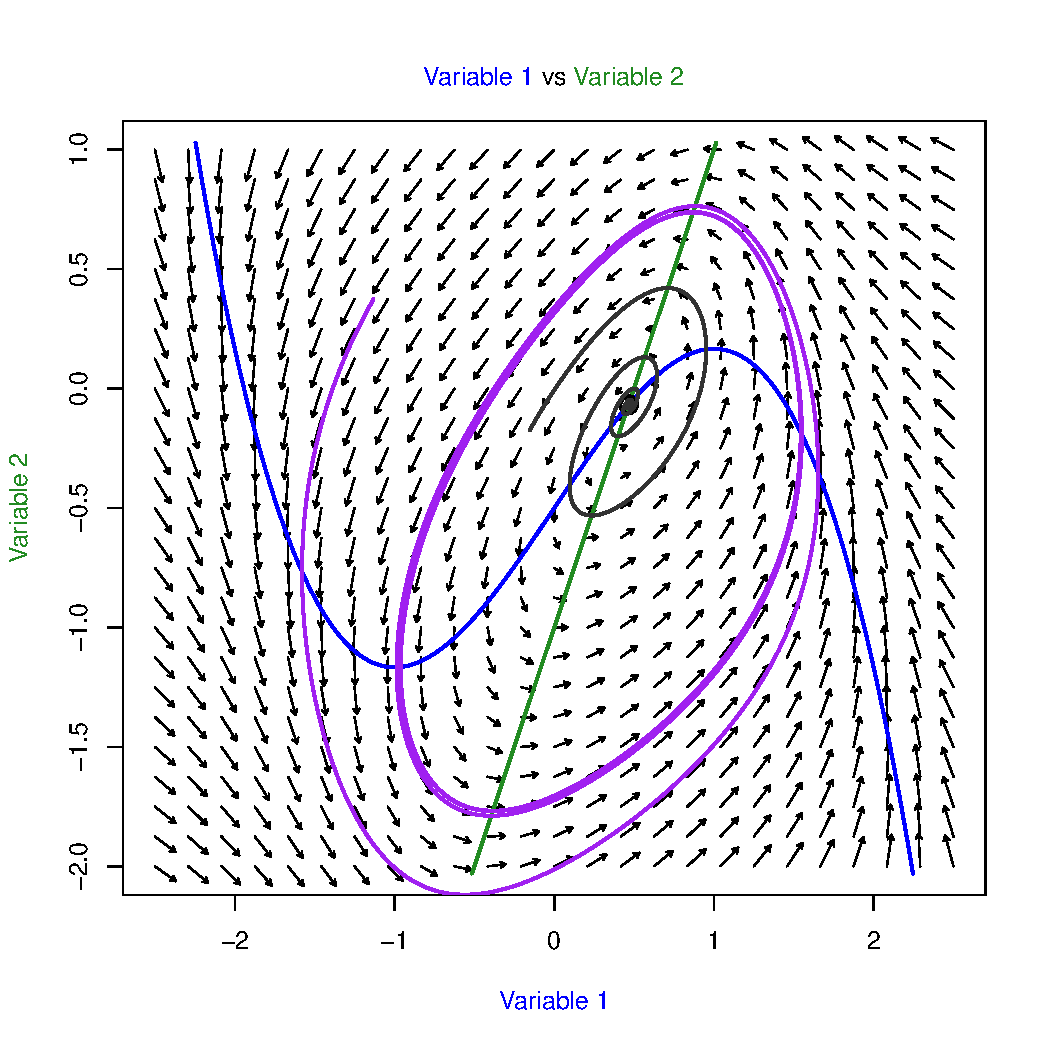
\includegraphics[width=4in]{figures/FHN-test-phase.pdf}}
\caption{Phase portrait of FHN system with $(a,b,c,j) = (-0.5, 0.5, 1, -0.5)$}
\label{fig:fhn-phase}
\end{figure} 

\textbf{Exercise \exnumber} Compute (and turn in) a complete phase portrait for the 
system with $(a,b,c,j)$ = (-0.5, 1.25, 2, -0.45), showing 
\begin{itemize}
 \item The equilibrium points and their stability.
 \item Any limit cycles and their stability.
 \item The limit sets of the stable and unstable manifolds of any saddles.
\end{itemize}

\begin{table}[tbp]
\centerline{
\begin{tabular}{||l|r|r|r|r|r|r|r|r|}
\hline
$a$ & -0.5 &-0.5 &-0.5 & -0.5 & -0.5 & -0.5 & -0.5 & -0.5\\ \hline
$b$ & 1.25 & 1.25 &1.25 & 1.25 & 1.25 & 1.25 & 1.25 & 1.25 \\ \hline
$c$ &    3 & 3 &  3 &    3 &    2 & 1.95 & 1.948 & 1.945 \\ \hline
$j$ & -0.5 & -0.49 & -0.48 & -0.45 & -0.45 & -0.45 & -0.45 & -0.45 \\ \hline
\end{tabular}}
\caption{Eight sets of parameter values for FHN system}
\label{fhn_table}
\end{table}

\textbf{Exercise \exnumber} Compute phase portraits for the parameter values given in Table \ref{fhn_table}. 
Turn in a write-up that identifies exactly what type of bifurcation (or bifurcations) occur between 
the parameter values in each successive pair of columns, and what components  
(equilibria, periodic orbits, limit sets of stable and unstable manifolds of a saddle point) 
differ for each pair of phase portraits. For example, you might contrast two successive
phase portraits by saying ``There is a saddle-node bifurcation, which results in the disappearance of two equilibria''. 
Note that only one parameter changes between each successive pair of columns, 
so the bifurcations that happen in this exercise will be of the types discussed in lecture. $\maltese$



%\begin{itemize}
%       \item Hopf bifurcation with appearance of periodic orbit
%       \item saddle-node bifurcation with appearance of two new equilibria
%       \item subcritical Hopf bifurcation produces unstable periodic orbit
%       \item homoclinic bifurcation destroys unstable periodic orbit
%       \item homoclinic bifurcation: unstable periodic orbit reappears, now surrounding all equilibrium points
%       \item saddle-node of limit cycles destroys both periodic orbits
%\end{itemize}

\textbf{Exercise \exnumber} For which sets of parameter values in the table is the system bistable? 
(Bistability means there are two distinct stable limit sets, not necessarily equilibrium points. A saddle point is not 
stable.) $\maltese$  

\section{Simulating the dynamics of spatial pattern formation} 

In this section we will study how the reaction-diffusion mechanism can create dynamic patterns
in space. As an example, we will use a system of equations where the reaction mechanism is the
Fitzhugh-Nagumo model, which is an approximation to the Hodgkin-Huxley equations for the
action potential in nerve cells. So that $x$ and $y$ can be used for spatial coordinates, we use
$u$ and $v$ for the state variables (note that $e$ here corresponds to $1/c$ in the previous
section, and the applied current $j$ is absent): 
\begin{equation}
\begin{aligned}
\frac{\partial u}{\partial t} & = \frac{1}{e}(u-\frac{u^3}{3} - v) +
D \left ( \frac{\partial^2 u}{\partial x^2} + \frac{\partial^2 u}{\partial y^2} \right )\\
\frac{\partial v}{\partial t} & = e(u + b - 0.5v)
\end{aligned} 
\label{sfnmodel} 
\end{equation}
In the electrophysiology interpretation of the model, $v$ represents the gating variable of an ion channel 
(fraction of open channels), which does not move; $u$ represents the membrane potential, which changes due 
to the combined effects of transmembrane currents (ion flow) and diffusion of ions in the tissue (which could 
be the surface of the heart, or (in one space dimension) a nerve axon). The model therefore has diffusion in $u$ but 
not in $v$, which is the extreme limit of the differing diffusion constants that are required for pattern formation 
by the Turing mechanism. 

\subsection{Finite difference approximation}
The simplest way to get approximate numerical solutions of equation \eqref{sfnmodel} is to 
discretize both space and time, replacing the derivatives in the equations by finite difference approximations. 
To explain this approach in the simplest setting, consider \emph{one-dimensional} diffusion, 
\begin{equation}
\frac{du}{dt} = D \frac{\partial^2 u}{\partial x^2}, \quad 0 \le x \le 1, 0 \le t \le T
\label{eqn:1D}
\end{equation}
with initial conditions $u(x,0)=u_0(x)$. For the spatial derivatives, we break up the interval $[0,1]$ 
into $m$ cells of width $k=1/m$, centered at the \emph{mesh points} 
$$ x_i = (i - 0.5)k, \quad i=1,2,\cdots, m. $$ 
To estimate the second spatial derivative, note that 
\begin{equation} 
\frac{u(x_{i+1},t) - u(x_{i},t)}{k} 
\label{eqn:rightSide}
\end{equation} 
is a finite-difference approximation to $\partial u/\partial x$ at the point halfway between $x_i$ and $x_{i+1}$. 
Similarly, 
\begin{equation} 
\frac{u(x_{i},t) - u(x_{i-1},t)}{k} 
\label{eqn:leftSide}
\end{equation} 
is an approximation to $\partial u/\partial x$ at the point halfway between $x_{i-1}$ and $x_i$. 
The difference between \eqref{eqn:rightSide} and \eqref{eqn:leftSide}, divided by $k$, is therefore an approximation 
to $\partial^2 u/\partial x^2$ at $x_i$. That is,  
\begin{equation}
\begin{aligned} 
\frac{\partial^2 u}{\partial x^2}(x_i,t) \approx 
& \frac{[u(x_{i+1},t)- u(x_i,t)]/k - [u(x_{i},t) - u(x_{i-1},t)]/k}{k} \\
= & \frac{u(x_{i+1},t) + u(x_{i-1},t) - 2u(x_i,t)}{k^2} 
\end{aligned} 
\label{eqn:2ndDeriv}
\end{equation} 

Note that both the first and second derivatives are estimated by a \emph{centered difference} approach, 
\begin{equation}
f'(x) \approx \frac{f(x+\varepsilon)-f(x-\varepsilon)}{2 \varepsilon}. 
\label{eqn:centered}
\end{equation}
The Taylor series $f(x \pm \varepsilon) = f(x) \pm \varepsilon f'(x) + \frac{1}{2}\varepsilon^2 f''(x) + O(\varepsilon^3)$ 
shows that the centered difference \eqref{eqn:centered} equals $f'(x) + O(\varepsilon^3)$. In contrast, the  
one-sided difference $\frac{f(x+\varepsilon)-f(x)}{\varepsilon}$ equals $f'(x) + O(\varepsilon^2)$, so 
centered differences are more accurate for small $\varepsilon$. 

You may be wondering: what do we do at $x_1$ and $x_m$, where \eqref{eqn:2ndDeriv} involves the nonexistent $x_0$ and $x_{m+1}$?
Recall that the solution to a system of partial differential equations depends on the boundary conditions -- what we assume about 
conditions at and beyond the boundary of the spatial domain. The boundary conditions that are most often encountered in practice
determine the values at the mesh points $x_0$ and $x_{m+1}$ that are outside the spatial domain. 

For our FHN example, we will consider \emph{no flux} boundary conditions: no material should flow out 
of the domain due to diffusion. The terms $[u(x_{i+1},t)- u(x_i,t)]$ and $[u(x_{i},t) - u(x_{i-1},t)]$ in the first line
of \eqref{eqn:2ndDeriv} represent net material flowing between two spatial cells. To make this flow zero at the domain 
boundaries $x=0,x=1$, we apply the finite-difference approximation \eqref{eqn:2ndDeriv} with $u(x_0,t)=u(x_1,t)$ 
and $u(x_{m+1},t)=u(x_m,t)$ for all $t$. Using those values, we can compute  \eqref{eqn:2ndDeriv} at all of the mesh
points inside the spatial domain (i.e., $x_1$ to $x_m$). 

\textbf{Exercise \exnumber} What should we do if the boundary conditions are that $u(x,t) \equiv 0$ for $x$ outside $[0,1]$? 
What should we do for \emph{periodic} boundary conditions $u(0,t) \equiv u(1,t)$?  $\maltese$ 

For the time derivatives, let $h$ be the time step for solutions of \eqref{eqn:1D} -- that is, we want 
values of $u(x_i,t)$ at times $t=0,h,2h,\cdots$. To accomplish this we can use \emph{Euler's method} which 
is based on the estimate 
\begin{equation}
\frac{\partial u}{\partial t}(x,t) \approx \frac{u(x,t+h) - u(x,t)}{h} \; \Rightarrow \; u(x_i,t+h) \approx u(x_i,t) + h \frac{\partial u}{\partial t}.(x_i,t)
\label{eqn:Euler}
\end{equation} 
Applying \eqref{eqn:Euler} and \eqref{eqn:2ndDeriv} to \eqref{eqn:1D} at the mesh points $x_i$, we get  
\begin{equation} 
\begin{aligned}
u(x_i,t+h) & \approx u(x_i,t) + h D \frac{\partial^2 u}{\partial x^2} \\
& \approx  u(x_i,t) + h D   \frac{u(x_{i+1},t) + u(x_{i-1},t) - 2u(x_i,t)}{k^2}.
\end{aligned}
\label{eqn:1DEuler}
\end{equation}  
Starting from the initial conditions $u(x_i,0) = u_0(x_i)$, applying \eqref{eqn:1DEuler} at all mesh 
points gives an approximate solution at time $h$. Starting from there, we do the same again to get an approximate 
solutionat time $2h$, and so on. 

\subsection{General method of lines} 
The solution method \eqref{eqn:1DEuler} consists of three steps:
\begin{enumerate}
\item Space is discretized so that the model only ``lives'' at a set of mesh points $x_i$.
\item Values of state variables at the grid points are used to approximate the spatial derivatives 
in the dynamic equations \eqref{sfnmodel}. 
\item We numerically solve the system of ODEs that result from steps 1 and 2. 
\end{enumerate}
This general approach is called the \textit{Method of Lines}. This name comes from imagining a set of lines
running forward in time, one based at each grid point, along which we solve the ODEs. 
In \eqref{eqn:1DEuler} we used evenly-spaced mesh points for step 1, finite-difference approximation 
for step 2, and Euler's method for step 3. All of those choices favor simplicity over efficiency, and more 
accurate results can be gotten with a bit more work. 

Step 3 can be done with a more accurate method for solving systems of ODEs. 
Substituting \eqref{eqn:2ndDeriv} into the model (equation \eqref{eqn:1D}) we have the (approximate) system
of ODEs 
\begin{equation} 
\frac{d u(x_i,t)}{dt} = D   \frac{u(x_{i+1},t) + u(x_{i-1},t) - 2u(x_i,t)}{k^2}.
\label{eqn:1DLines}
\end{equation}
We can then get numerical solutions with any method for solving systems of ODEs -- in principle. In practice, the
systems resulting from finite-difference approximations to PDEs are often hard to solve numerically, as we discuss below. 

Step 2 can be done more accurately using \textit{spectral methods} (Trefethen 2000).
Spectral methods do a spatial interpolation of each state variable at each time point, fitting a smooth function that 
matches the current values at the mesh points. Spatial derivates of the fitted function are 
used as the approximate spatial derivatives of the state variable. Spectral
methods generally use unevenly spaced mesh points, and the best choice of mesh points and 
interpolating function depends on the spatial domain and boundary conditions. Spectral methods can be very
efficient because the entire {(interpolate+differentiate)} process can be expressed as a single
matrix multiplication, with a matrix that is computed once and then used at all time steps. 
See Trefethen (2000) for an introduction and pointers to more advanced treatments.  

Spectral methods are an efficient way to get high-accuracy solutions on a simple spatial domains,  
but it is usually necessary to use an implicit or semi-implicit ODE solver (Trefethen 2000). 
For the complex spatial domains that often arise in engineering applications, other methods are needed that start 
by breaking up a complex domain into a set of simpler domains. In general, apart from simple PDEs on simple domains  
(such as the ones in this document), it is better to step outside \R and use 
specialized software for numerical solution of PDEs. 

\subsection{Spatial Fitzhugh-Nagumo}
The script \texttt{sfn.R} uses the finite-difference approach on the spatial Fitzhugh-Nagumo model
\eqref{sfnmodel} in a rectangulr domain with no flux boundary conditions. For two spatial dimensions, 
we break up space into an \ttt{nx} by \ttt{ny} grid of square cells with side $k$, and put a mesh point at the center of each cell
(rectangular cells could be used instead). To apply the no-flux boundary conditions, we surround the domain by a ``ring'' of sites where the
state variables take the same values as those at the adjacent site (in the $x$ or $y$ direction) in the interior of the domain. 
Using this trick, the following \R function calculates the right hand side of the finite-difference approximation for 
the right-hand side of \eqref{sfnmodel}:
\blst
sfn=function(u,v) {
   ny = dim(u)[1]; nx = dim(u)[2];
   uec = cbind(u[,1],u,u[,nx]); # u with extra columns
   uer = rbind(u[1,],u,u[ny,]); # u with extra rows 
   ul = uer[3:(ny+2),]+uer[1:ny,]+uec[,1:nx]+uec[,3:(nx+2)]-4*u;
   uf = (u-0.3333*u*u*u-v)/e + dx2*ul;
   vf = e*(u + b - 0.5*v);
   return(list(uf=uf,vf=vf)); 
} 
\end{lstlisting}
\ttt{ul} is the finite difference approximation to  $\dfrac{\partial^2 u}{\partial x^2}  + \dfrac{\partial^2 u}{\partial y^2}$ that
results from applying \eqref{eqn:2ndDeriv} in both the $x$ and $y$ directions, and \texttt{dx2} is value of $D/k^2$.  

An important practical feature is that there are \textit{no loops} in \ttt{sfn}. 
Everything is written as matrix operations, making the calculations much faster. 
Simulating the system is still quite slow; loops would make it intolerable. 

As in the example of 1-dimensional diffusion, we use Euler's method for the time derivatives:
\blst
sfn.run=function(nsteps,init) {
   u=init$u; v=init$v; 
   for (i in 1:nsteps){
      out = sfn(u,v);
      u = u + h*out$uf;	v = v + h*out$vf;
      if (i%%5 == 1) image(1:dim(u)[2],1:dim(u)[1],t(u),col=rainbow(n=1000,start=0,end=0.7))
      cat(i,"\n"); 
   }
   return(list(u=u,v=v)); 
}
\end{lstlisting} 
Because each time step depends on the results from the previous step, we \textit{do} need a for-loop to 
iterate the model over time. The value returned by \ttt{sfn.run} is the final state of the model, suitable for use as 
a new ``initial condition'' to continue the run. 

The script {\texttt sfn.R} includes everything needed to produce and plot simulations of the model. 
First, select and run the block of code with the functions \ttt{sfn} and \ttt{sfn.run}. Then select and
run the code for the first parameter set/initial condition at the bottom of the script. 
The commands
\blst
pdf(file="sfn.pdf",onefile=TRUE);
nsteps=1000; # or however many time steps you want 
out=sfn.run(nsteps,init1);
dev.off();
\end{lstlisting}
run the model with the first parameters and initial conditions for 1000 iterations, and save an image of the
system state to a PDF file every 5 time steps. To continue the model run, you can use \ttt{sfn.run} again, 
starting from the model state at the last time step:
\blst
out=sfn.run(nsteps,out)
\end{lstlisting} 

\textbf{Exercise \exnumber} Here are some exercises you can do with the {\texttt sfn.R} script:
\begin{itemize}
\item[(a)] Restart the model using the second set of parameters and initial conditions, and see what happens
when spiral waves collide with with one another. 
\item [(b)] Experiment with changing the spatial discretization parameter $k$. What
effect do you expect to see on the spatial pattern?
\item[(c)] Experiment with \textit{gradually} increasing the time step $h$. You should discover that
solutions quickly go from reasonable to nonsensical, or that the computation crashes. It is characteristic
of explicit solution methods that very small values of $h$ are needed to keep numerical solutions of PDEs 
from developing errors that grow exponentially fast (``explicit'' means that the set of values at the next time step 
is a computable function of the values at the current time; in ``implicit'' methods
the values at the next time step are the solution to a system of nonlinear equations, which must be found numerically). $\maltese$   
\end{itemize} 

The script \ttt{sfnLines.R} uses Method of Lines to solve the spatial Fitzhugh Nagumo model by Method of Lines. The  
order-4 Runga-Kutta method is used to solve the ODE system, by re-writing the {sfn} function so it can be 
used with the \ttt{rk4} function. Because \ttt{rk4} is an explicit method like Euler's method, it still requires short 
time steps, but it gives more accurate solution of the ODE system. Only implicit solution methods, such as the widely used
Crank-Nicholson method, remain numerically stable for long time steps. 

\textbf{Exercise \exnumber} Modify \ttt{sfnLines.R} to generate numerical solutions of the 
Klausmeier (1999) model for pattern formation in vegetation on hillsides in semiarid regions. A nondimensionalized 
version of the model is: 
\begin{equation} 
\begin{aligned}
\frac{\partial w}{\partial t} & = a - w - w n^2 + v \frac{dw}{dx} \\
\frac{\partial n}{\partial t} & = w n^2  - mn + \frac{\partial^2 n}{\partial x^2} + \frac{\partial^2 n}{\partial y^2}
\end{aligned}
\end{equation}
Here $w$ is water and $n$ is vegetation. In the $w$ equation 
$a>0$ represents supply rate (rainfall), $wn^2$ is uptake by plants and $-w$ is
other loss processes; $v dw/dx$ is downhill (leftward) flow of water at velocity $v$. 
In the $n$ equation $wn^2$ is vegetation growth, $mn$ is vegetation mortality, and the diffusion
term represents local expansion of vegetated areas through growth of established plants and new recruits that establish in
the neighborhood of their parents. 

Have your script simulate the model on a $60 \times 60$ grid of square cells of side \texttt{dx=dy=1} (physically, these
are 1 m$^2$ cells) with parameter values $a=2, v=80, m=0.5$. Use periodic boundary conditions in both $x$ and $y$, that is
$$u(0,y,t) = u(60,y,t), \quad u(x,0,t)=u(x,60,t).$$ 
In other respects, use the same methods as in \ttt{sfnLines.R} for generating the approximate numerical 
solution of this model. 

For initial conditions: if \ttt{nx=60} is the number of grid cells in each direction, use 
\blst 
n0=seq(0,1,length=nx); n0=(4*n0*(1-n0))^2; 
n0 = 0.5+0.25*outer(n0,n0); 
w0 = matrix(parms["a"],nx,nx); 
image(1:nx,1:nx,t(n0)/max(n0),main="Vegetation",col=rainbow(n=1000,start=0,end=0.7)); 
\end{lstlisting} 
The initial water concentration \ttt{w0} is the steady state in the absence of vegetation; the last line above shows you what the
initial vegetation pattern is. You will need to use a short time step ($h=0.01$, for example) to get valid solutions. $\maltese$  

\textbf{Exercise \exnumber} What pattern does the model produce, if you let it run long enough? (If you have not run it long enough,
you can continue a simulation by taking the final state as your new initial conditions). Turn in a script that runs ``long enough''
and a plot illustrating the pattern that forms. $\maltese$ 

\textbf{Exercise \exnumber} Write a script that explores the question: is the final pattern sensitive to initial conditions, 
or do you find the same behavior in the long run regardless of what initial conditions you choose? 
Remember that the initial conditions have to satisfy the periodic boundary conditions, and only consider initial conditions
where vegetation is not completely absent. $\maltese$ 

\textbf{Exercise \exnumber} Write a script to explore the question: 
how does the final pattern change as parameters $a,v,m$ are changed? 
Experiment by making small changes in these, one at a time, and determining what the 
effects are. For example, do things happen faster or slower? 
Do biologically interesting features become larger, smaller, or disappear? $\maltese$ 

\section{References}
Chambers, J.M. and T.J. Hastie. 1992. Statistical Models in S. Chapman and Hall, London. 

Chambers, J.M. 1998. Programming with Data. Springer, New York. 

Ermentrout, B. 2002. Simulating, Analyzing, and Animating Dynamical Systems: A Guide to XPPAUT for Researchers and Students. SIAM (Society for Industrial and Applied Mathematics), Philadelphia. 

Fussmann, G., S.P. Ellner, K.W. Shertzer, and N.G. Hairston, Jr. 2000. 
Crossing the Hopf bifurcation in a live predator-prey system. Science 290: 1358-1360. 

Gardner, T.S., C.R. Cantor and J.J. Collins. 2000. Construction of a genetic
toggle switch in {\it Escherichia coli}. Nature 403: 339-342. 

Ihaka, R., and R. Gentleman. 1996. R: a language for data analysis and graphics.
Journal of Computational and Graphical Statistics 5: 299- 314. 

Kelley, C.T. Iterative Methods for Optimization. SIAM (Society for Industrial
and Applied Mathematics), Philadelphia PA. 

Klausmeier, C.A. 1999. Regular and irregular patterns in semiarid vegetation.
Science 284: 1826-1828. 

Maindonald, J. H. 2004. Using \R for Data Analysis and Graphics: Introduction,
Code, and Commentary. URL \texttt{http://www.cran.R-project.org}.

R Core Team (2017). R: A language and environment for statistical
computing. R Foundation for Statistical Computing, Vienna, Austria.
ISBN 3-900051-07-0, URL \texttt{http://www.R-project.org/.}

Trefethen, L. 2000. Spectral Methods in MATLAB. SIAM (Society for Industrial
and Applied Mathematics), Philadelphia. 

Venables, W.N. and B.D. Ripley. 2000. S Programming. Springer, New York. 

Venables, W.N. and B.D. Ripley. 2002. Modern Applied Statistics with S (4th edition). Springer, New York. 

Verzani, J. 2002. \textsf{simpleR} -- using \R for Introductory Statistics. 
URL \texttt{http://www.cran.R-project.org}.

\end{document}
